%%%%%%%%%%%%%%%%%%%%%%%%%%%%%%%%%%%%%%%%%
% Masters/Doctoral Thesis 
% LaTeX Template
% Version 2.5 (27/8/17)
%
% This template was downloaded from:
% http://www.LaTeXTemplates.com
%
% Version 2.x major modifications by:
% Vel (vel@latextemplates.com)
%
% This template is based on a template by:
% Steve Gunn (http://users.ecs.soton.ac.uk/srg/softwaretools/document/templates/)
% Sunil Patel (http://www.sunilpatel.co.uk/thesis-template/)
%
% Template license:
% CC BY-NC-SA 3.0 (http://creativecommons.org/licenses/by-nc-sa/3.0/)
%
%%%%%%%%%%%%%%%%%%%%%%%%%%%%%%%%%%%%%%%%%

%----------------------------------------------------------------------------------------
%	PACKAGES AND OTHER DOCUMENT CONFIGURATIONS
%----------------------------------------------------------------------------------------

\documentclass[
12pt, % The default document font size, options: 10pt, 11pt, 12pt
%oneside, % Two side (alternating margins) for binding by default, uncomment to switch to one side
french, % ngerman for German
singlespacing, % Single line spacing, alternatives: onehalfspacing or doublespacing
%draft, % Uncomment to enable draft mode (no pictures, no links, overfull hboxes indicated)
%nolistspacing, % If the document is onehalfspacing or doublespacing, uncomment this to set spacing in lists to single
liststotoc, % Uncomment to add the list of figures/tables/etc to the table of contents
%toctotoc, % Uncomment to add the main table of contents to the table of contents
parskip, % Uncomment to add space between paragraphs
%nohyperref, % Uncomment to not load the hyperref package
headsepline, % Uncomment to get a line under the header
%footsepline,
%chapterinoneline, % Uncomment to place the chapter title next to the number on one line
%consistentlayout, % Uncomment to change the layout of the declaration, abstract and acknowledgements pages to match the default layout
]{MastersDoctoralThesis} % The class file specifying the document structure

\usepackage[utf8]{inputenc} % Required for inputting international characters
\usepackage[T1]{fontenc} % Output font encoding for international characters

\usepackage{mathpazo} % Use the Palatino font by default

% "biblatex" DOESN'T WORK TOGETHER WITH "thebibliography"
% See https://tex.stackexchange.com/a/277744/160548
%\usepackage[backend=bibtex, style=authoryear, natbib=true]{biblatex} % Use the bibtex backend with the authoryear citation style (which resembles APA)
%\addbibresource{example.bib} % The filename of the bibliography

%----------------------------------------------------------------------------------------
% FRENCH TRANSLATIONS added by me
%----------------------------------------------------------------------------------------

\providecaptionname{french}{\acknowledgementname}{Remerciements}
\providecaptionname{french}{\abbrevname}{Liste des abréviations}

%----------------------------------------------------------------------------------------
% PACKAGES, SETTINGS AND COMMANDS added by me
%----------------------------------------------------------------------------------------
\usepackage{minted} % for code syntaxing
\usepackage[colorinlistoftodos,prependcaption,textsize=tiny,obeyFinal]{todonotes}
\usepackage{pdfpages}
\usepackage{xargs}  % Use more than one optional parameter in a new command
\usepackage{scrextend} % Add support for labeling lists. See https://en.wikibooks.org/wiki/LaTeX/List_Structures#Some_special_lists
\usepackage{subcaption} % Add support for subfigure

\usepackage[autostyle=true]{csquotes} % Required to generate language-dependent quotes in the bibliography

\captionsetup{width=0.8\textwidth}

%---- Improved figure caption ----
%  Add the possibility to have a different text in the list of figures, 
% and to easily add a source.
%Source: https://tex.stackexchange.com/a/251299/160548
\usepackage{xparse}
\NewDocumentCommand{\captionsource}{omm}{%
  \IfNoValueTF{#1}
   {% no leading optional argument
    \caption[#2\formatsource{#3}]{#2}%
   }
   {% leading optional argument
    \caption[#1\formatsource{#3}]{#2}%
   }
}
\NewDocumentCommand{\formatsource}{m}{%
  \unskip\ (Source:~\cite{#1})%
}
%----------------------------------------------

%\newcommand\sourcecaption[2]{\caption[#2 \protect\cite{#1}]{#2}}

\newcommand{\keyword}[1]{\textbf{#1}}
\newcommand{\tabhead}[1]{\textbf{#1}}
\newcommand{\code}[1]{\texttt{#1}}
\newcommand{\file}[1]{\texttt{\bfseries#1}}
\newcommand{\option}[1]{\texttt{\itshape#1}}
% uncomment to see an exemple
%\keyword{keyword}
%\code{code}
%\file{file}
%\option{option}

\newcommandx{\unsure}[2][1=]{\todo[linecolor=red,backgroundcolor=red!25,bordercolor=red,#1]{#2}}
\newcommandx{\change}[2][1=]{\todo[linecolor=blue,backgroundcolor=blue!25,bordercolor=blue,#1]{#2}}
\newcommandx{\info}[2][1=]{\todo[linecolor=OliveGreen,backgroundcolor=OliveGreen!25,bordercolor=OliveGreen,#1]{#2}}
\newcommandx{\improvement}[2][1=]{\todo[linecolor=plum,backgroundcolor=plum!25,bordercolor=plum,#1]{#2}}
\newcommandx{\thiswillnotshow}[2][1=]{\todo[disable,#1]{#2}}
%----------------------------------------------------------------------------------------
%	MARGIN SETTINGS
%----------------------------------------------------------------------------------------

\geometry{
	paper=a4paper, % Change to letterpaper for US letter
	inner=2.5cm, % Inner margin
	outer=3.8cm, % Outer margin
	bindingoffset=.5cm, % Binding offset
	top=1.5cm, % Top margin
	bottom=1.5cm, % Bottom margin
	%showframe, % Uncomment to show how the type block is set on the page
}

%----------------------------------------------------------------------------------------
%	THESIS INFORMATION
%----------------------------------------------------------------------------------------

\thesistitle{Visionneuse améliorée de modèles 3D pour la planification territoriale} % Your thesis title, this is used in the title and abstract, print it elsewhere with \ttitle
\supervisor{Paul \textsc{Albuquerque}} % Your supervisor's name, this is used in the title page, print it elsewhere with \supname
\examiner{} % Your examiner's name, this is not currently used anywhere in the template, print it elsewhere with \examname
%\degree{Doctor of Philosophy} % Your degree name, this is used in the title page and abstract, print it elsewhere with \degreename
\author{Michaël \textsc{Polla}} % Your name, this is used in the title page and abstract, print it elsewhere with \authorname
\addresses{} % Your address, this is not currently used anywhere in the template, print it elsewhere with \addressname

\subject{Computer Sciences} % Your subject area, this is not currently used anywhere in the template, print it elsewhere with \subjectname
\keywords{} % Keywords for your thesis, this is not currently used anywhere in the template, print it elsewhere with \keywordnames
\university{\href{http://hepia.hesge.ch}{Hepia}} % Your university's name and URL, this is used in the title page and abstract, print it elsewhere with \univname
\department{option Ingénierie logicielle} % Your department's name and URL, this is used in the title page and abstract, print it elsewhere with \deptname
\group{Technologies de l’information et de la communication} % Your research group's name and URL, this is used in the title page, print it elsewhere with \groupname
\faculty{Faculty Name} % Your faculty's name and URL, this is used in the title page and abstract, print it elsewhere with \facname

\AtBeginDocument{
\hypersetup{pdftitle=\ttitle} % Set the PDF's title to your title
\hypersetup{pdfauthor=\authorname} % Set the PDF's author to your name
\hypersetup{pdfkeywords=\keywordnames} % Set the PDF's keywords to your keywords
\hypersetup{colorlinks=false} % See the FAQ (AppendixA.tex) or https://tex.stackexchange.com/a/50754/160548 for color configuration
}

\begin{document}

\frontmatter % Use roman page numbering style (i, ii, iii, iv...) for the pre-content pages

\pagestyle{plain} % Default to the plain heading style until the thesis style is called for the body content

%----------------------------------------------------------------------------------------
%	TITLE PAGE
%----------------------------------------------------------------------------------------
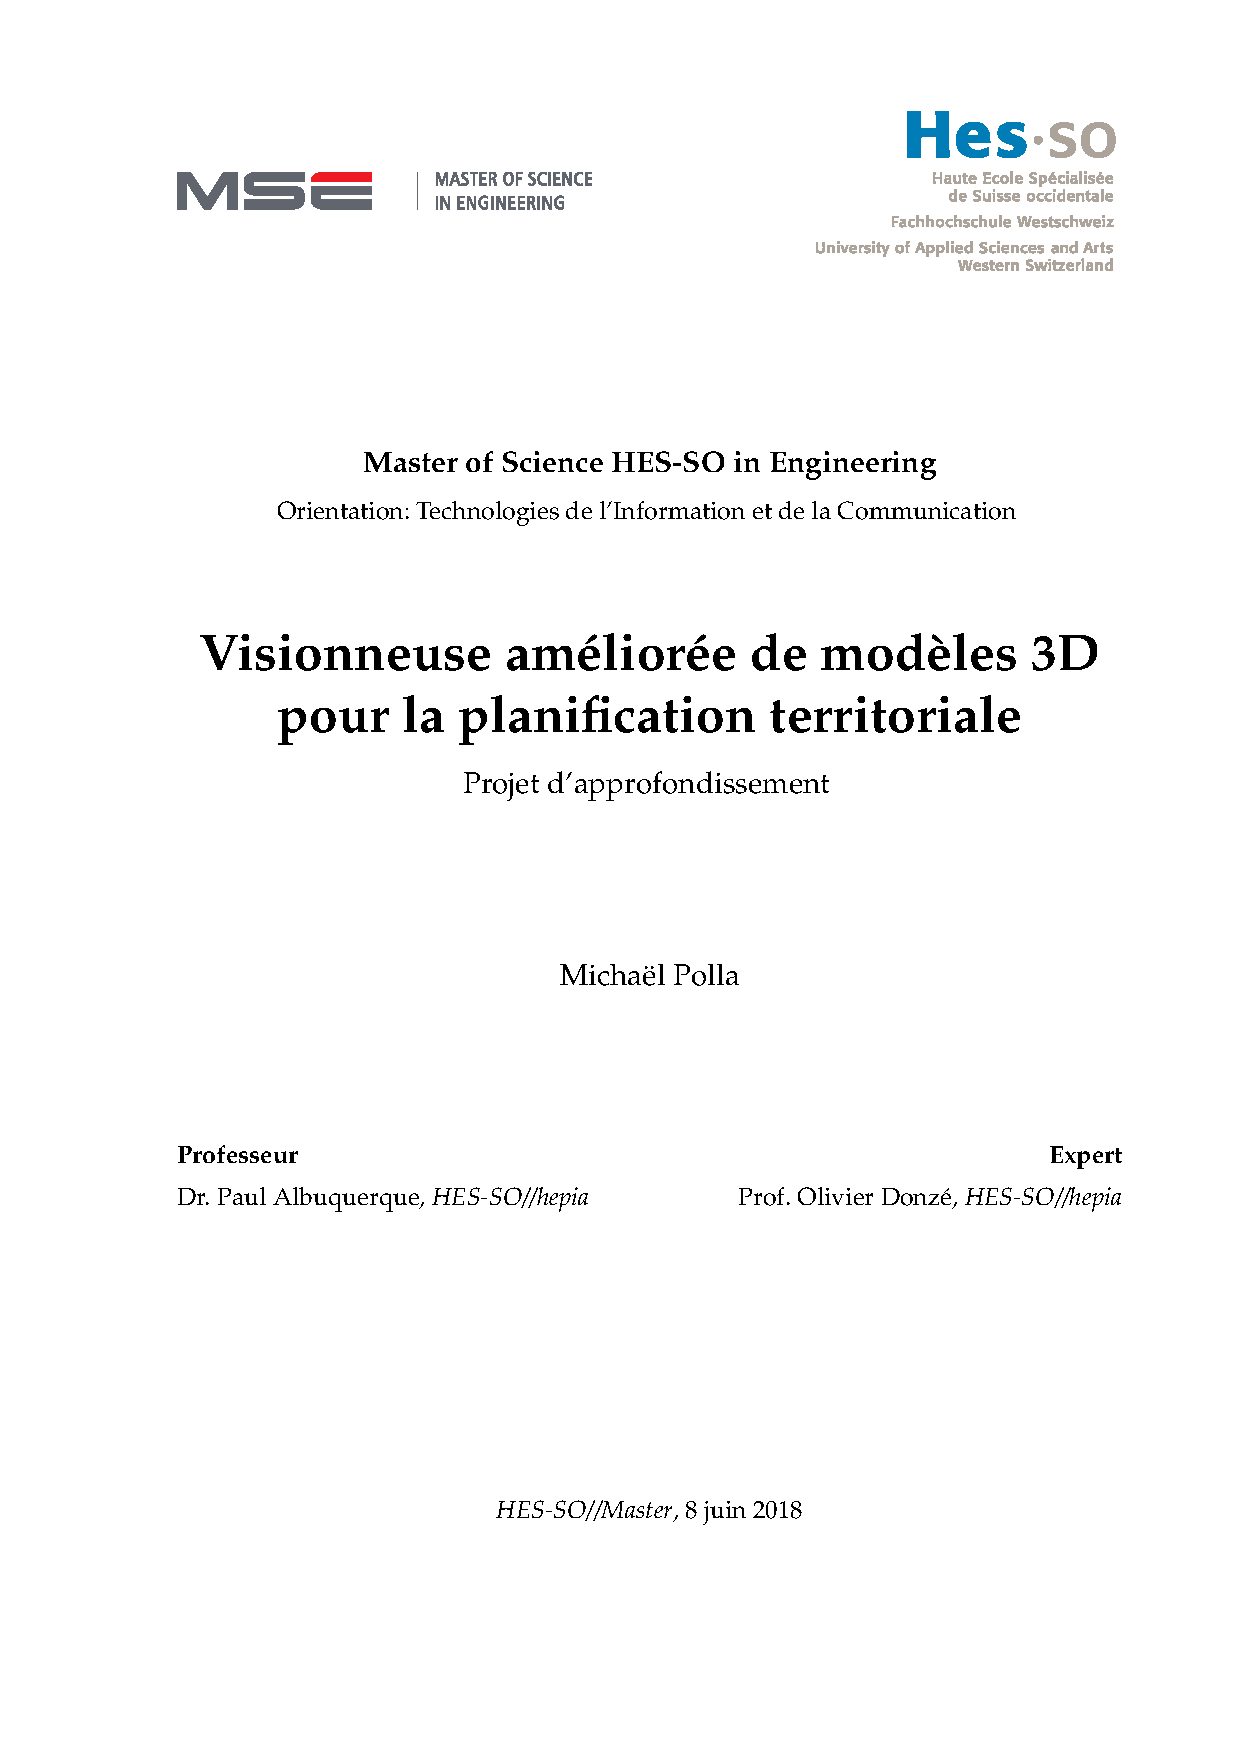
\includepdf[pages=-]{Chapters/CoverPages.pdf}

%\begin{titlepage}
%\begin{center}

%\vspace*{.06\textheight}
%{\scshape\LARGE \univname\par}\vspace{1.5cm} % University name
%\textsc{\Large Projet d'approfondissement HES-SO}\\[0.5cm] % Thesis type

%\HRule \\[0.4cm] % Horizontal line
%{\huge \bfseries \ttitle\par}\vspace{0.4cm} % Thesis title
%\HRule \\[1.5cm] % Horizontal line
 
%\begin{minipage}[t]{0.4\textwidth}
%\begin{flushleft} \large
%\emph{Auteur :}\\
%\authorname % Author name - remove the \href bracket to remove the link
%\end{flushleft}
%\end{minipage}
%\begin{minipage}[t]{0.5\textwidth}
%\begin{flushright} \large
%\emph{Professeur~HES~responsable~:} \\
%\supname % Supervisor name - remove the \href bracket to remove the link  
%\end{flushright}
%\end{minipage}\\[3cm]
 
%\vfill

%\large
%\textbf\groupname\\\deptname\\[2cm] % Research group name and department name
 
%\vfill

%{\large Printemps 2018}\\[4cm] % Date
%\includegraphics{Logo} % University/department logo - uncomment to place it
%\vfill
%\end{center}
%\end{titlepage}

%----------------------------------------------------------------------------------------
%	PROJECT SUMMARY (external page)
%----------------------------------------------------------------------------------------

%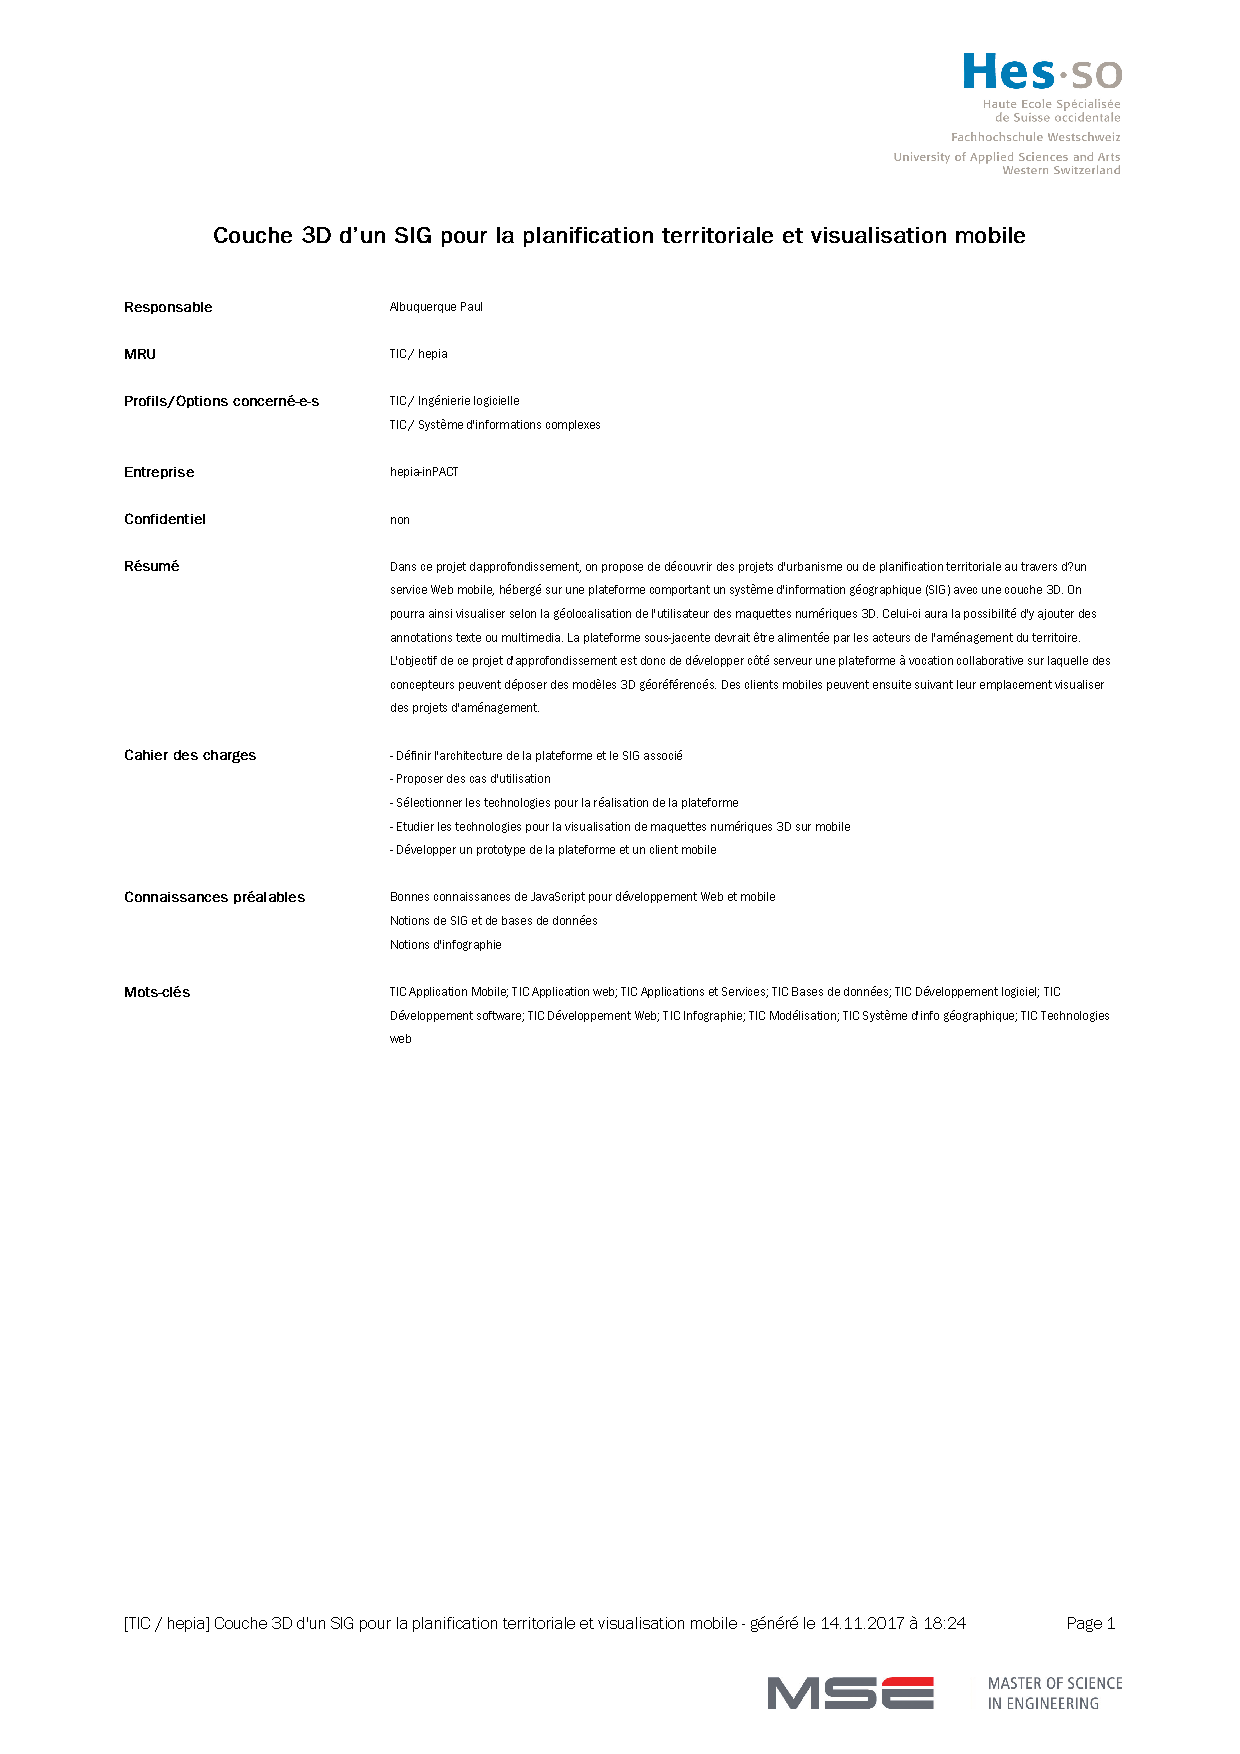
\includepdf[pages={1}]{Figures/project-description.pdf}
%\clearpage
%----------------------------------------------------------------------------------------
%	ACKNOWLEDGEMENTS
%----------------------------------------------------------------------------------------
\begin{acknowledgements}
\addchaptertocentry{\acknowledgementname} % Add the acknowledgements to the table of contents
Tout d'abord, je tiens à remercier mon professeur responsable, Paul Albuquerque, ainsi qu'Olivier Donzé, pour la confiance qu'ils m'ont accordée pour ce projet d'approfondissement, leurs conseils avisés et leur disponibilité. J'ai vraiment apprécié réaliser ce travail. J'ai également apprécié \todo{synonyme} la passion et le plaisir de partager ses connaissances de M. Donzé.

Je remercie également mes collègues et amis Maxime Burri, Salvatore Cicciù et Michaël Minelli pour leur présence, leur soutien sans faille, et tous les bons moments passés en ensemble. Avoir fait leur connaissance est l'une des meilleures choses que ces études m'auront apportées. Pas sûr que j'aurais tenu autant de semestres sans vous !

Enfin, je remercie de tout mon coeur ma femme Mélanie, pour les innombrables raisons qui font que je l'aime. Pas un jour ne passe sans que je pense à la chance que j'ai de t'avoir dans ma vie. Merci d'exister et d'être qui tu es.

\end{acknowledgements}

%----------------------------------------------------------------------------------------
%	LIST OF CONTENTS/FIGURES/TABLES PAGES
%----------------------------------------------------------------------------------------

\tableofcontents % Prints the main table of contents

\listoffigures % Prints the list of figures

%\listoftables % Prints the list of tables

%----------------------------------------------------------------------------------------
%	ABBREVIATIONS
%----------------------------------------------------------------------------------------

\begin{abbreviations}{ll} % Include a list of abbreviations (a table of two columns)

\textbf{API} & \textbf{A}pplication \textbf{P}rogramming \textbf{I}nterface \\
\textbf{BIM} & \textbf{B}uilding \textbf{I}nformation \textbf{M}odeling \\
\textbf{ISO} & \textbf{I}nternational \textbf{O}rganization for \textbf{S}tandardization \\
\textbf{GPU} & \textbf{G}raphics \textbf{P}rocessing \textbf{U}nit \\
\textbf{JSON} & \textbf{J}ava\textbf{S}cript \textbf{O}bject \textbf{N}otation \\
%\textbf{glTF} & \textbf{GL} \textbf{T}ransmission \textbf{F}ormat \\
\textbf{PaaS} & \textbf{P}latform \textbf{a}s \textbf{a} \textbf{S}ervice \\
\textbf{PLQ} & \textbf{P}lan \textbf{L}ocalisé de \textbf{Q}uartier \\
\textbf{SIG} & \textbf{S}ystème d'\textbf{I}nformation \textbf{G}éographique \\
\textbf{WYSIWYG} & \textbf{W}hat \textbf{Y}ou \textbf{S}ee \textbf{I}s \textbf{W}hat \textbf{Y}ou \textbf{G}et \\

\end{abbreviations}

%----------------------------------------------------------------------------------------
%	THESIS CONTENT - CHAPTERS
%----------------------------------------------------------------------------------------

\mainmatter % Begin numeric (1,2,3...) page numbering

\pagestyle{thesis} % Return the page headers back to the "thesis" style

% Include the chapters of the thesis as separate files from the Chapters folder
% Uncomment the lines as you write the chapters

\chapter{Introduction}

\label{Chapter1} % For referencing the chapter elsewhere, use \ref{Chapter1} 

La présentation de projets d'urbanisme ou de planification territoriale auprès du public a toujours été un défi. 

Depuis son apparition, la CAO aide les professionnels du domaine à réaliser des modélisations toujours plus précises et réalistes. 
Malheureusement, le partage de ces modélisations nécessite généralement de créer plusieurs maquettes 3D et de les mettre à disposition. Cela demande d'autant plus de travail et de temps que le projet est complexe, voire inclut différentes étapes (2 ans, 5 ans...) avec en conséquence une multitude de maquettes à réaliser.

\begin{figure}[h]
    \centering
    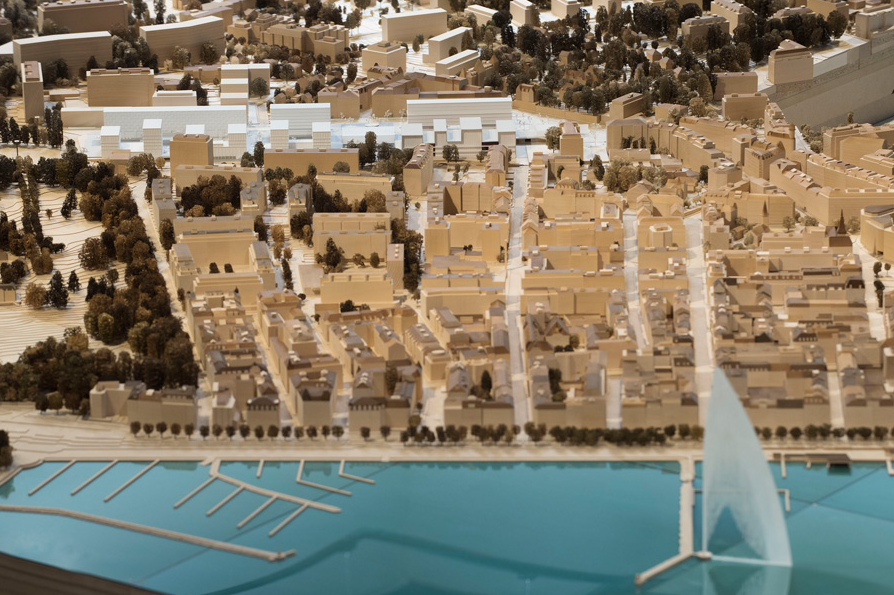
\includegraphics[width=0.8\linewidth]{Figures/geneva-model.png}
    \caption{Maquette de la ville de Genève réalisée à la main.}
    \label{fig:geneva-model}
\end{figure}

L'avènement des imprimantes 3D a permis de réduire cette charge de travail, tout en produisant des maquettes plus fidèles. 


\begin{figure}[h]
    \centering
    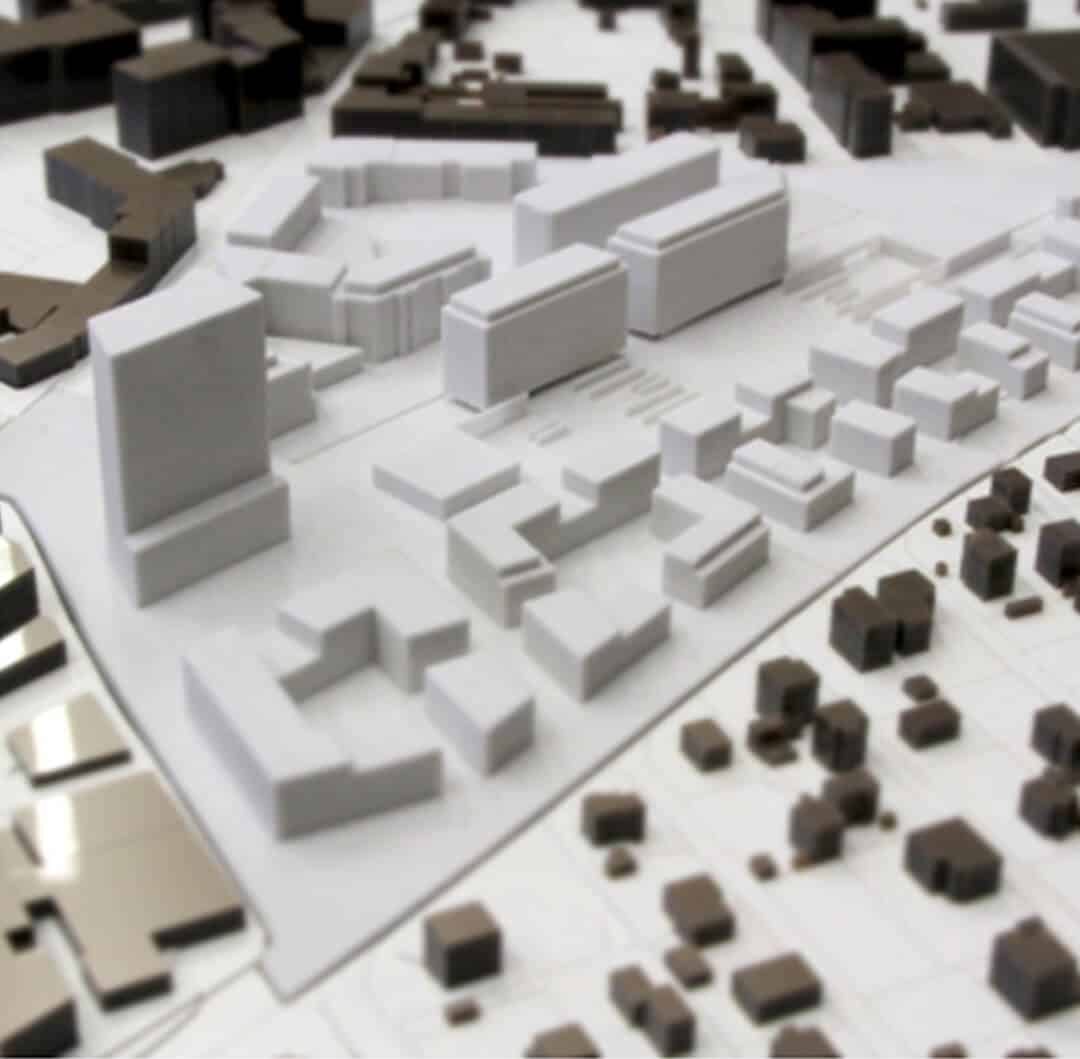
\includegraphics[width=0.5\linewidth]{Figures/3d-printed-model.jpg}
    \captionsource{Exemple de maquette imprimée en 3D.}{3d-printed-model}
    \label{fig:3d-printed-model}
\end{figure}

Un autre problème survient alors: pour voir lesdites maquettes, il faut se rendre à l'endroit où elles sont exposées.

Une solution à cela serait le partage direct des modèles réalisés à l'ordinateur avec les personnes concernées. Cependant, la majorité des projets sont créés à l'aide de logiciels propriétaires, dont la licence est bien souvent très coûteuse (AutoCAD, SketchUp, Cinema4D...). Il n'est dès lors pas envisageable d'exiger des utilisateurs un tel investissement d'argent et de temps (installation, configuration) dans un simple but de consultation des projets.
Bien que certains de ces produits proposent gracieusement une visionneuse, celle-ci est généralement limitée aux formats supportés par l'éditeur.

Fort heureusement, des outils gratuits permettant de visualiser des modèles 3D de toutes sortes, ont fait leur apparition sur le marché ces dernières années. Certains sont proposés gracieusement par les éditeurs des produits cités précédemment, à l'instar d'Autodesk Viewer. D'autres sont des logiciels clients, comme la visionneuse 3D fournie d'office avec Windows 10 ou Open 3D Model Viewer\footnote{\url{www.open3mod.com}}. Enfin, des solutions en ligne sont également disponibles. Celles-ci ont l'avantage de n'exiger aucune installation, et d'être accessibles à la majorité des systèmes d'exploitation, ne nécessitant qu'un navigateur internet.
C'est cette dernière catégorie qui nous intéresse dans le cadre de ce projet.

Parmi les outils en ligne existants, le plus utilisé, et sans doute le plus complet actuellement, se nomme \textbf{Sketchfab}. Plus qu'une simple visionneuse, il s'agit d'une plateforme permettant de stocker, partager et visualiser des modèles 3D. 
%Elle sera détaillée dans la section \ref{sketchfab}.

\section{Sketchfab} \label{sketchfab}

Lancée en 2012, Sketchfab\footnote{\url{www.sketchfab.com}} est une plateforme web d'hébergement de contenus 3D, ne ciblant aucune catégorie particulière : cela va des modèles de petits objets de la vie courante, de personnages, aux modélisations de paysages et lieux complexes.

\begin{figure}
    \centering
    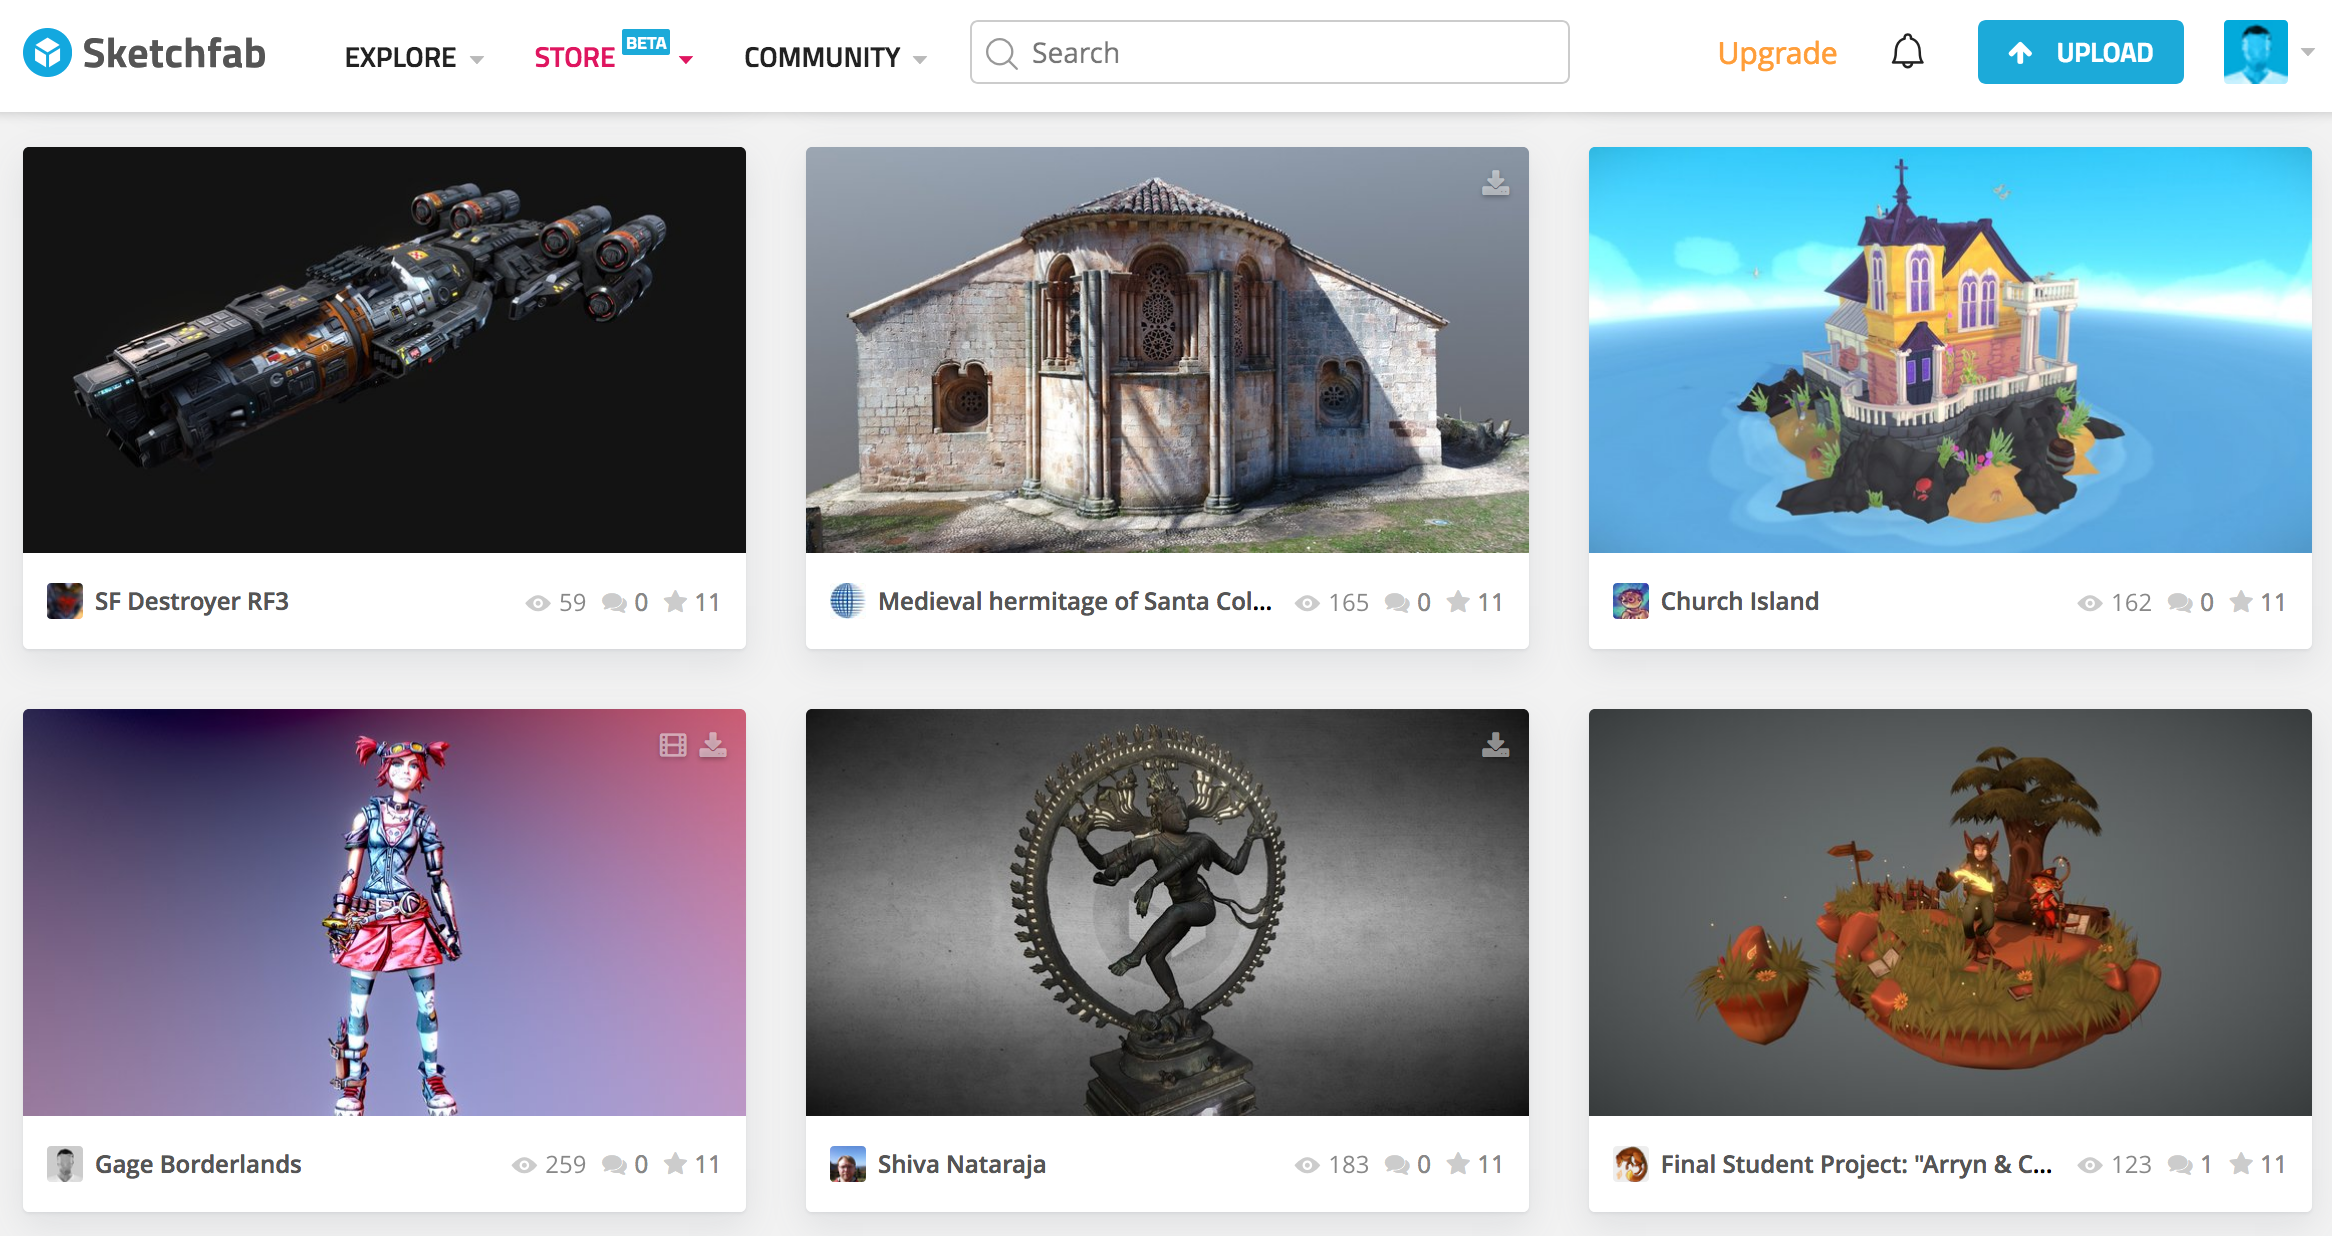
\includegraphics[width=\linewidth]{Figures/sketchfab-overview.png}
    \caption{Affichage de modèles récemments ajouté à Sketchfab.}
    \label{fig:sketchfab-overview}
\end{figure}

Elle permet de visualiser les modèles 3D sur toutes plateformes possédant un navigateur (ordinateurs, smartphones, et même casques de réalité virtuelle).
Il est ainsi possible de naviguer dans le modèle à l'aide d'une souris ou de manière tactile, selon le support. Les opérations "classiques" telles que \textit{zoomer} ou \textit{pivoter} sont disponibles.
Le propriétaire d'un modèle peut également lui adjoindre des annotations. Une annotation est liée à une coordonnée 3D choisie sur le modèle, possède un titre, et peut contenir un texte descriptif ou une image.

\begin{figure}[h]
    \centering
    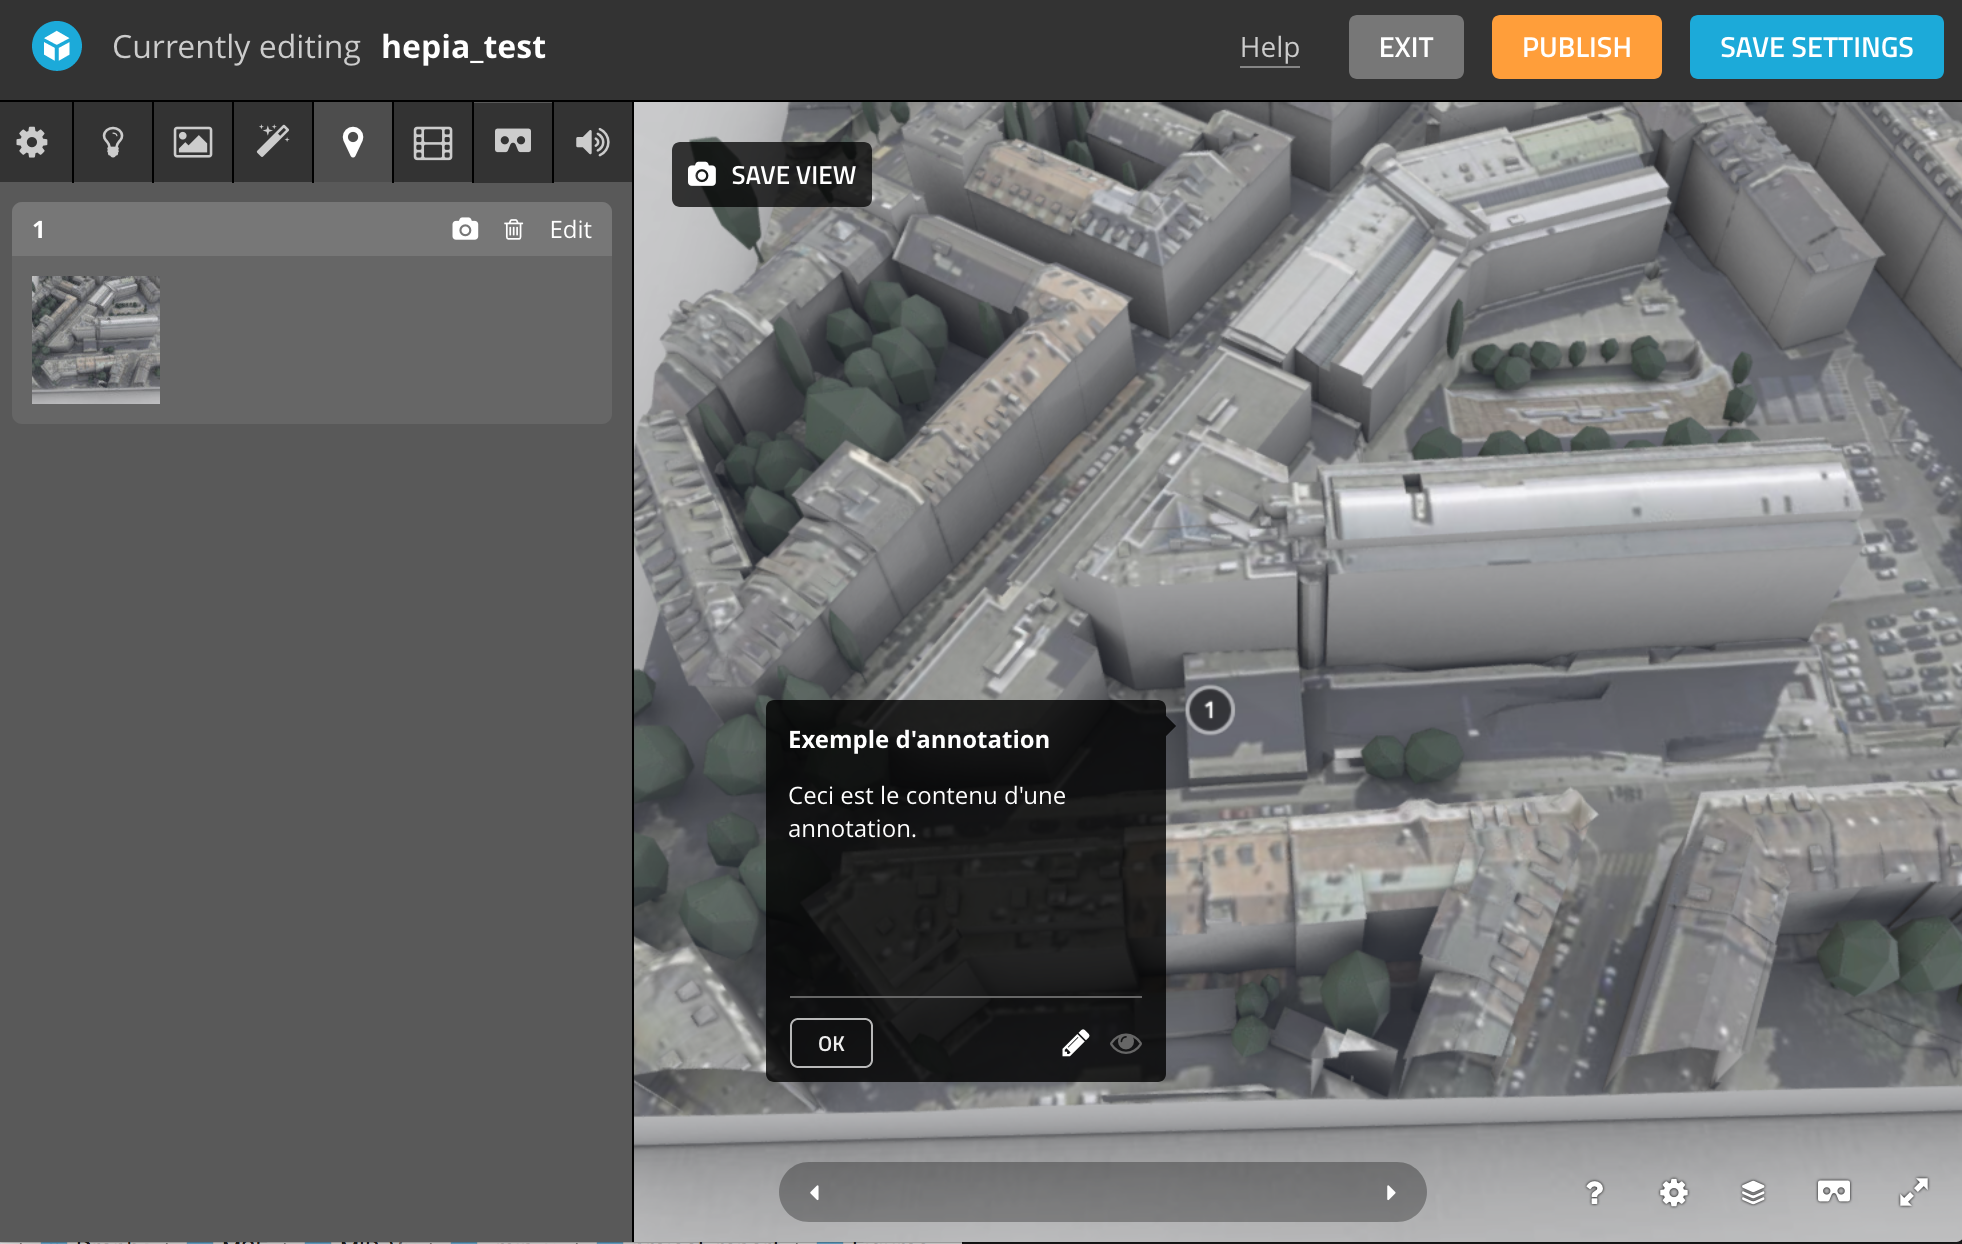
\includegraphics[width=\linewidth]{Figures/sketchfab-annotation-example.png}
    \caption{Ajout d'une annotation à un modèle dans Sketchfab.}
    \label{fig:sketchfab-annotation-example}
\end{figure}

Sketchfab propose plusieurs niveaux de fonctionnalités \footnote{\url{https://sketchfab.com/plans}}. Les principales limitations de l'offre gratuite sont:
\begin{itemize}
    \item Les modèles ajoutés sont obligatoirement référencés et publiques; il n'est pas possible d'en restreindre l'accès.
    \item La taille maximale d'un modèle est de 50 Mo, contre plusieurs centaines de Mo avec une offre payante, ce qui est assez restreignant.
    \item Seules 5 annotations peuvent être ajoutées à un modèle.
\end{itemize}

Récemment, la plateforme a mis en place un \textit{store} (encore en version \textit{beta}) permettant de vendre et acheter des modèles, généralement un peu plus complexes et travaillés.

\section{Problématique}

À la Haute école du paysage, d'ingénierie et d'architecture de Genève (hepia), le groupe de modélisation informatique du paysage\footnote{Groupe MIP, institut inPACT, \url{https://mip.hesge.ch}} (MIP) manifeste un intérêt marqué pour un tel outil dans le cadre de ses mandats. En intégrant une telle plateforme dans ses processus, le partage et l'accès aux modélisations pour les acteurs concernés s'en trouveraient facilité.

\textit{Sketchfab} présente néanmoins des lacunes. Pour commencer, citons les limitations évoquées dans la section~\ref{sketchfab}, malgré l'option plus ou moins satisfaisante de la formule payante.
S'agissant d'une plateforme généraliste, elle n'offre pas certains outils spécifiques, propres au domaine de l'urbanisme. D'autres inconvénients, comme le manque de personnalisation (par exemple, pouvoir isoler les divers modèles relatifs à un projet), les droits d'accès (gérer les personnes autorisées à consulter un groupe de modèles, ainsi que les possibilités d'interactions de chacun).

Concernant les annotations, rappelons que leur nombre est limité à cinq pour la formule gratuite, et qu'elles ne peuvent contenir que du texte et des images (celles-ci devant alors être hébergées ailleurs). En outre, la description ne peut dépasser 1024 caractères.

Idéalement, il faudrait pouvoir bénéficier d'une plateforme similaire à \textit{Sketchfab}, mais répondant aux besoins spécifiques du domaine de l'aménagement du territoire, tout en offrant la possibilité d'être aisément personnalisable.

\section{Objectifs}

Le but général du présent projet est d'étudier la faisabilité et les problématiques de mise en place d'une telle plateforme à vocation collaborative.

Suite à des discussions avec le Prof. Olivier Donzé pour cibler les besoins du groupe MIP, et en tenant compte du temps limité à disposition, l'accent est mis sur les tâches suivantes:
\begin{itemize}
    \item Définir l'architecture de la plateforme.
    \item Déterminer et présenter des cas d'utilisation.
    \item Rechercher et étudier les solutions existantes qui pourraient servir à composer les différentes "briques" du logiciel.
    \item Etudier les technologies de visualisation de maquettes numériques 3D.
    \item Réaliser, si possible, un prototype ou des illustrations à des fins démonstratives.
\end{itemize}

L'architecture se voudra modulaire, afin de pouvoir bien distinguer chaque composant fonctionnel.

Enfin, les possibilités concernant les annotations, notamment le contenu qu'elles peuvent proposer, seront mises en évidence. 
Il s'agit en effet d'un outil particulièrement pratique, et souvent évoqué lors des dicussions autour du sujet de ce travail.

\section{Réalisation}

Le résultat de ce travail est une étude appronfondie des différentes briques pouvant composer une plateforme de modélisation 3D avec gestion d'annotations, destinée particulièrement au secteur de l'urbanisme.

Pour chaque fonctionnalité, des recherches ont été réalisées afin de découvrir si des solutions libres existaient, notamment sur les principaux dépôts de code comme \textit{GitHub} ou \textit{GitLab}. Le cas échéant, celles-ci ont été analysées (librairies et technologies utilisées) afin de déterminer dans quelle mesure il serait envisageable de les utiliser, en association avec d'autres, pour rapidement implémenter un prototype démontrant la faisabilité de mise en place d'une telle plateforme.

Une version de démonstration a justement été développée afin d'illustrer cette utilisation de modules existants et les possibilités d'améliorations éventuelles. Un bilan et des perspectives d'évolution sont également disponibles et viennent ainsi compléter le démonstrateur.

\begin{figure}[h]
    \centering
    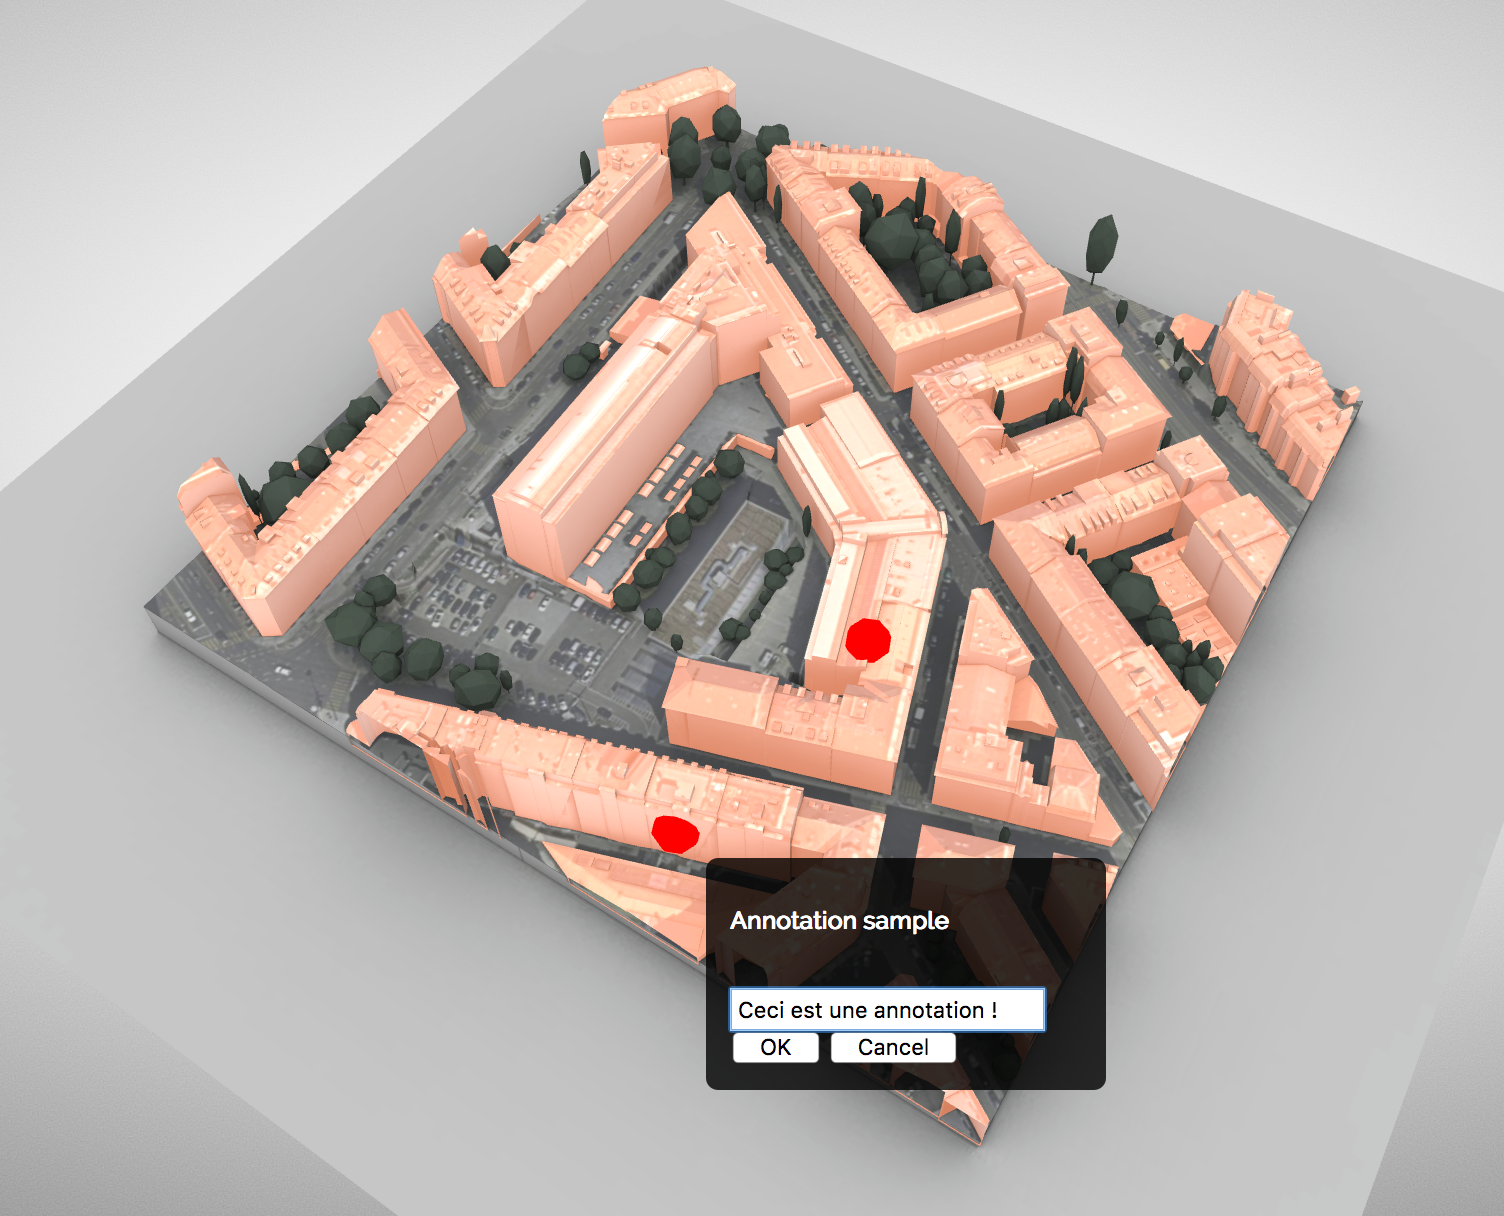
\includegraphics[width=\linewidth]{Figures/mip-viewer-overview.png}
    \caption{"MIP-Viewer", le prototype réalisé: ajout d'annotation sur un modèle importé.}
    \label{fig:mip-viewer-overview}
\end{figure}

L'ensemble du projet (prototype, rapport, illustrations...) est disponible sur GitHub à l'adresse : \textbf{\url{https://github.com/MichaelPolla/mip-viewer/}}


\chapter{Analyse préliminaire}
\label{Chapter2}

Lors des séances préparatoires, le Prof. Olivier Donzé a décrit différentes situations réelles qui pourraient bénéficier d'une plateforme Web embarquant une visionneuse de modèles 3D avec annotations possibles, et de quelle façon celle-ci pourrait être mise à contribution.

Cela a permis d'une part d'identifier les différents groupes d'utilisateurs potentiels et leurs besoins respectifs, et d'autre part les fonctionnalités qui pourraient être mises à leur disposition. On procède donc à une analyse des besoins suivie par une analyse fonctionnelle.

\section{Besoins métiers}
\label{sec:requirements-analysis}

L'une des situations évoquées est le concours d'architecture, prenant par exemple place suite à l'adoption d'un plan localisé de quartier (PLQ)\footnote{Exemple : "Concours d'architecture sur le périmètre de la gare CEVA des Eaux-Vives" \cite{plq-contest}}.
Un tel événement regroupe les principaux acteurs de l'urbanisme, et est par conséquent une situation intéressante à analyser.

Voici une description des différentes catégories d'utilisateurs :

\textbf{Participants} \\
Pour réaliser leur projet, les participants ne partent généralement pas de rien, mais doivent prendre en compte des bâtiments et structures déjà existants. Et même si ce n'est pas le cas (zone destinée à être rasée), il faut que leur réalisation s'intègre à l'environnement avoisinant.

Une fois leur travail réalisé, celui-ci, avec d'éventuels documents annexes, doit être transmis aux personnes concernées afin d'être jugé.

\textbf{Experts} \\
Les experts effectuent une sorte de présélection, en vérifiant que les propositions répondent aux critères imposés. Ils émettent d'éventuels commentaires, à destination du jury notamment.

\textbf{Membres du jury} \\
Le jury établit le classement parmi les projets ayant passé la phase de présélection. Leur apprécation ne nécessite pas un niveau de détail aussi fourni que pour les experts. Ils peuvent adjoindre des remarques aux travaux, par exemple pour indiquer ce qui a particulièrement retenu leur attention.

\textbf{Public restreint} \\
Il s'agit d'un nombre limité de personnes "du métier", par exemple des collaborateurs du service de l'urbanisme, qui vont consulter les résultats avant que ceux-ci ne soient rendus complètement publics.
Ils peuvent ajouter des informations à destination du grand public.

\textbf{Grand public} \\
Une fois les résultats connus, une exposition est mise en place afin que la population puisse admirer les projets retenus et s'informer grâce aux informations supplémentaires mises à leur disposition.

\begin{figure}[h]
    \centering
    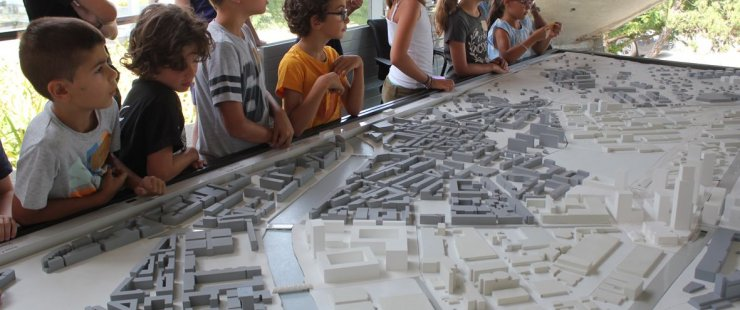
\includegraphics[width=\linewidth]{Figures/exposition-maquette-pav.jpg}
    \captionsource{Exposition de la maquette du projet Praille-Acacias-Vernets (PAV)}{pav}
    \label{fig:exposition-maquette-pav}
\end{figure}

Voici les principaux besoins qui ressortent de cette analyse:
\begin{itemize}
    \item Accéder à l'état actuel de la zone concernée (plans, maquettes...) ou au modèle sur lequel se baser. (\textit{Participants})
    \item Mettre les réalisations à disposition du comité du concours. (\textit{Participants})
    \item Consulter les modèles (\textit{Tous}, différents niveaux d'accès)
    \item Ajouter des informations au projet (\textit{Tous, excepté grand public})
    \item Consulter les informations ajoutées (\textit{Tous})
\end{itemize}

Le problème actuel est que l'accès aux informations d'origine, le rendu des projets, l'ajout de commentaires et leur communication entre les différents groupes ne sont pas toujours efficaces. De même, la consultation des modèles, comme évoqué en introduction, nécessite de savoir où, ou auprès de qui se rendre pour cela.

Pour ces raisons, un outil conçu à cet effet, accessible via le web, aurait de grands avantages.

\section{Fonctionnalités nécessaires}

Maintenant que les besoins ont été définis, il est possible d'imaginer les fonctionnalités que la plateforme pourrait offrir aux différents groupes :

\textbf{Participants} \\
Si le concours porte sur un modélisation existante, celle-ci peut leur être mise à disposition par ce biais.
Une fois réalisée, les participants déposent leurs créations sur la plateforme. On peut aussi imaginer que le système vérifie que les contraintes imposées aient été respectées, et que tous les éléments demandés aient bien été rendus.
Enfin, ils peuvent ajouter des annotations à leur modèle, par exemple pour donner plus d'information sur un élément ou joindre une photo. Ces annotations sont liées à des coordonnées spécifiques choisies.

\textbf{Experts} \\
Les experts ont un accès détaillé aux travaux des participants. Ils peuvent consulter les annotations des participants et, si nécessaire, en ajouter.

\textbf{Membres du jury} \\
Le jury a accès aux projets ayant passé la présélection. Il a accès à des fonctionnalités similaires que les experts. La vue proposée peut afficher des données plus générale que pour ces derniers.

\textbf{Public restreint} \\
Ces personnes consultent les résultats, visualisent les annotations ajoutées et peuvent en joindre d'autres, telles que des informations complémentaires sur telle ou telle "point" du modèle, destinées au grand public.

\textbf{Grand public} \\
La population peut consulter les travaux lauréats, et obtenir plus d'information en consultant les annotations associées à chacun.

Les fonctionnalités se résument ainsi :

\begin{itemize}
    \item Importation/Exportation de modèles 3D
    \item Consultation des modèles
    \item Ajout et lecture d'annotations
    \item Gestion des utilisateurs (droits d'accès)
\end{itemize}

Concernant les annotations, celles-ci visent différents buts tels que :
\begin{itemize}
    \item Un participant les utilise pour proposer des vues prédéfinies de différents points de son projet.
    \item Les experts les emploient pour émettre leurs remarques.
    \item Un membre du jury ajoute ses questions sur des points particuliers.
    \item Des annotations d'ordre général sont proposées au public.
\end{itemize}

\section{Architecture générale}
\label{sec:global-architecture}

Suite à ces analyses, une architecture générale, représentant les fameuses "briques" nécessaires à la réalisation de la plateforme et qui fourniront les fonctionnalités identifiées, peut être proposée.

Pour commencer, un \textit{mindmap} (Figure \ref{fig:mip-viewer-mindmap}) a été réalisé, afin d'identifier les modules qui pourraient composer l'outil.
Celui-ci a été dessiné avec \textit{Coggle}\footnote{\url{https://coggle.it/}}, une application web dédiée à cela.

\begin{figure}[h]
    \centering
    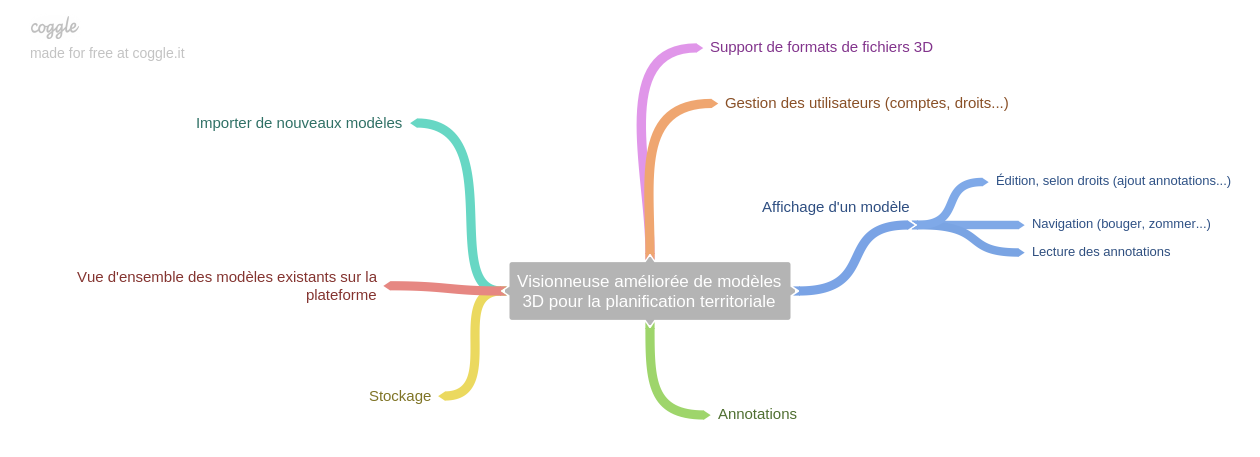
\includegraphics[width=\linewidth]{Figures/mip-viewer-mindmap.png}
    \captionsetup{width=0.9\textwidth}
    \caption{Résultat du \textit{Mind map} des modules imaginés pour l'application.}
    \label{fig:mip-viewer-mindmap}
\end{figure}

En ne considérant que les fonctionnalités qui nous intéresse dans le cadre de ce projet, nous pouvons constater que l'architecture générale existante de \textit{Sketchfab} peut être représentée de façon similaire.\todo{je sais pas si c'est utile, c'était pour dire qu'on n'est sur la bonne voie}

La figure \ref{fig:mip-viewer-components-interactions-diagram} présente cette fois de manière plus détaillée ces modules, en précisant les principales interactions entre ceux-ci.

\begin{figure}
    \centering
    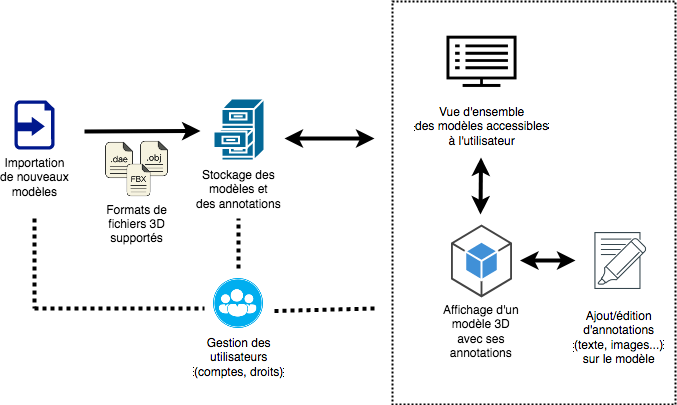
\includegraphics[width=0.9\linewidth]{Figures/mip-viewer-components-interactions-diagram.png}
    \caption{Les "briques" de l'outil et leurs principales interactions.}
    \label{fig:mip-viewer-components-interactions-diagram}
\end{figure}

L'analyse a également révélé l'importance des annotations. Celles-ci peuvent améliorer la communication et enrichir les modèles, avec la diversité de contenu qu'elles peuvent intégrer. La figure \ref{fig:various-media-for-annotation} illustre cela.

\begin{figure}
    \centering
    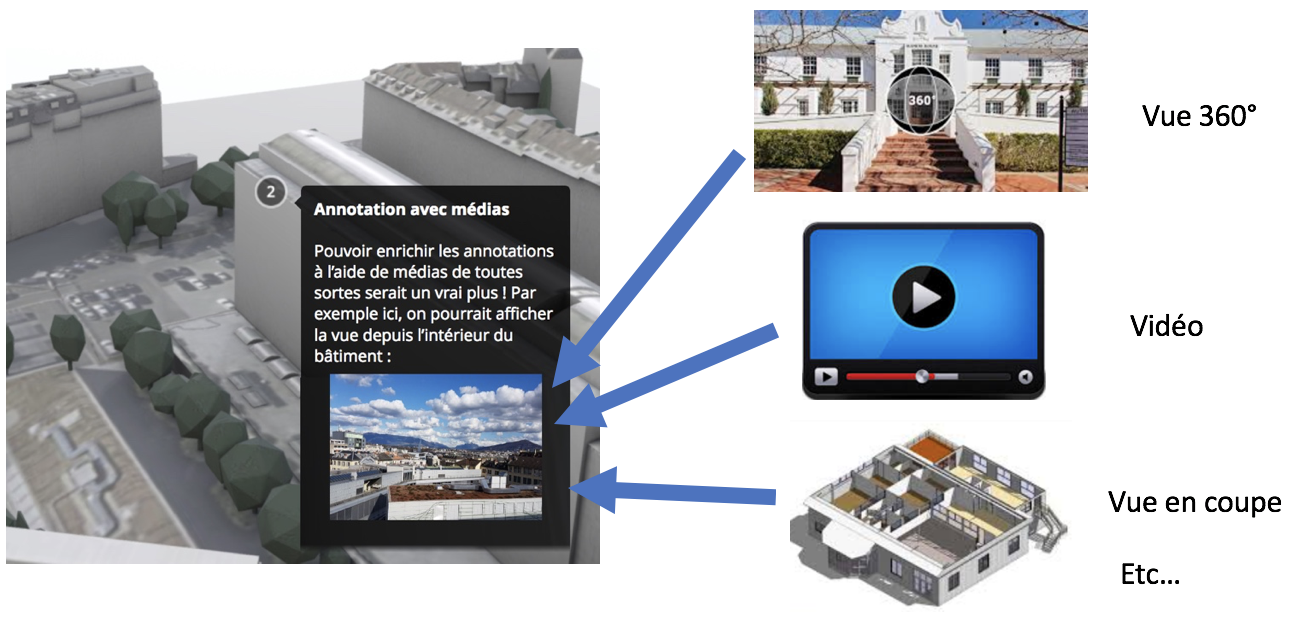
\includegraphics[width=\linewidth]{Figures/various-media-for-annotation.png}
    \caption{Exemples de différents médias qu'une annotation pourrait contenir.}
    \label{fig:various-media-for-annotation}
\end{figure}

Enfin, la plupart des fonctionnalités sont disponibles pour plusieurs, voire toutes, les catégories d'utilisateurs. Ces derniers ont cependant des accès différents, déterminant les actions qui leur sont autorisées. Par exemple, un jury pourra consulter certains modèles, mais ne pourra pas en ajouter, au contraire d'un architecte ou des participants au concours.

La figure \ref{fig:use-cases} en donne un exemple. Toute personne a accès en consultation aux modèles publiques et aux annotations associées à chacun d'eux. Un membre du jury ou équivalent pourra lui, en plus de cela, ajouter ou éditer des annotations. Enfin, un architecte ou similaire pourra également ajouter de nouveaux modèles.

\begin{figure}[ht]
    \centering
    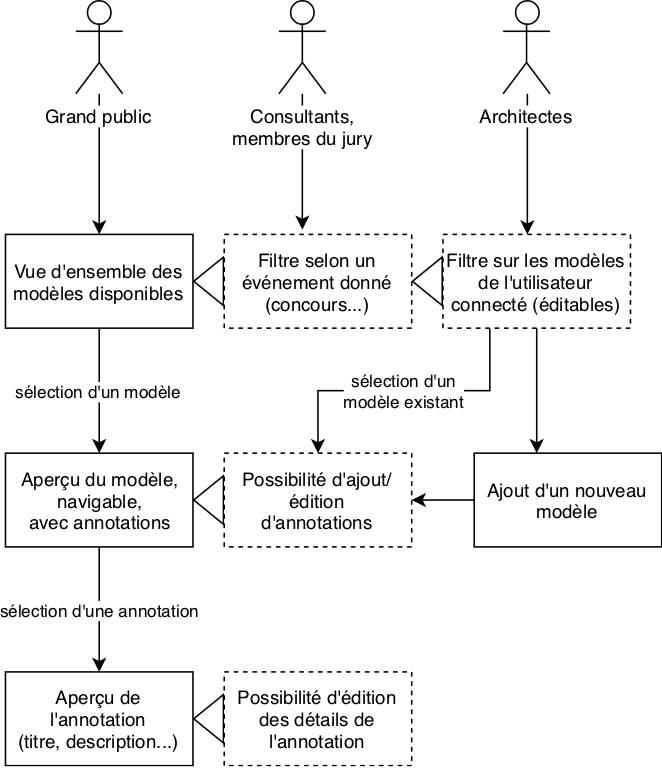
\includegraphics[width=0.6\linewidth]{Figures/use-cases.png}
    \caption{Exemples des niveaux d'accès aux fonctionnalités.}
    \label{fig:use-cases}
\end{figure}






 
\chapter{Technologies \& implémentations}
\label{Chapter3}

Ce chapitre reprend en détail chaque brique, en exposant pour chacune les recherches effectuées et des propositions de solutions pour leur implémentation ou mise en place.

\unsure{déplacer paragraphe ci-dessous ?}
Découvrant les domaines de l'urbanisme et de la modélisation du paysage avec la réalisation de ce projet, j'ai commencé par étudier les technologies et processus les plus répandus dans ces secteurs.
\todo{BIM \& CO ?}

\section{Formats de fichiers 3D}

Dans le cadre de la mise en place d'une plateforme de partage de modèles 3D, l'étude des formats de fichiers existants (usages, tendances, compatibilité...) est un point de départ intéressant. Cela permet tout d'abord de découvrir comment sont représentées les données de modélisation, et comment les manipuler. On prend également connaissance des logiciels principaux du marché.

Au final, cela aidera à décider quel(s) format(s) seraient à considérer pour notre outil, celui-ci devant pouvoir \textbf{supporter les formats les plus courants} afin d'être aisément utilisable.

Il existe plus d'une centaine de formats permettant de stocker des données tridimensionnelles. De nombreuses listes de ces derniers sont disponibles sur internet, mais la plupart ne mentionnent que les principaux formats. La section consacrée à cette catégorie de fichiers sur \textit{Wikipédia}\footnote{\url{https://en.wikipedia.org/wiki/List_of_file_formats\#3D_graphics}} s'avère être l'une des plus fournies. 

\todo{\url{https://www.archives.gov/files/applied-research/ncsa/8-an-overview-of-3d-data-content-file-formats-and-viewers.pdf}}

Cette abondance s'explique entre autres par la variété des domaines concernés : de la représentation de structure moléculaires (format XYZ\footnote{Spécifications du format \textit{XYZ} : \url{http://openbabel.org/wiki/XYZ_\%28format\%29}}), à la cryo-microscopie électronique (format MRC\footnote{Spécifications du format MRC : \url{http://www.ccpem.ac.uk/mrc_format/mrc2014.php}}), en passant par les formats de certains éditeurs de jeux ou consoles (\textit{MDX} chez \textit{Blizzard Entertainment},\textit{BDL} et \textit{BMD3} chez Nintendo...), et bien entendu tous les logiciels de modélisation/animation/CAD (\textit{Blend} pour \textit{Blender}, \textit{FBX}, \textit{MAX}, \textit{MB} et bien d'autres pour les différentes suites proposées par \textit{Autodesk}, \ldots).

Dans le cadre de ce projet, les formats qui nous intéressent sont bien entendu ceux qui concernent l'urbanisme, au travers des logiciels de CAO/DAO correspondants.

Enfin, il est important de savoir qu'un fichier 3D n'est pas qu'une simple liste de coordonnées 3-axes, mais contient généralement de nombreuses informations telles que : 
\begin{itemize}
    \item Caméras : types, emplacements, orientations...
    \item Lumières : types, emplacements, effets...
    \item Maillages (\textit{meshes}),
    \item Textures,
    \item Animations, sons...
\end{itemize}

Le contenu exact varie beaucoup d'un format à l'autre. Aussi, là où un certain format permettra de stocker l'ensemble des informations d'un modèle, un autre nécessitera de séparer les données (par exemple, un fichier pour le squelette, la lumière... et un autre pour les textures). \todo{Exemple concret} 

\todo{section dédiée à ce que contient un fichier 3D ?}

\subsection{Formats de fichiers de DAO/CAO courants}

Les formats les plus présents actuellement sont détaillés ci-après.

\subsubsection{FBX}
\textit{FBX} (\textbf{F}ilm\textbf{b}o\textbf{x}) est un format appartenant à \textit{Autodesk}.

Bien que propriétaire, une \textit{API}\footnote{\url{https://www.autodesk.com/products/fbx/overview}} fournit le nécessaire pour lire et écrire ces fichiers.

Il a été créé pour pallier les variétés de formats rencontrés dans le flux de travail, et ainsi assurer l'interopérabilité entre les produits d'\textit{Autodesk}, tels que \textit{3ds Max}, \textit{Maya} ou \textit{Motion Builder}, ainsi que de nombreux autres logiciels comme \textit{Cinema4D}, \textit{Rhino} ou \textit{Unity3D}.

De fait, cela en fait un format populaire, très répandu.
Une rapide recherche sur \textit{GitHub}\footnote{\url{https://github.com/search?q=fbx+viewer}} nous renvoie de nombreux projets de visionneuses \textit{FBX}.

\subsubsection{OBJ}
\textit{OBJ} est un format libre très utilisé pour transférer des informations d'une application à l'autre. Il s'agit d'un format de données simple, en \textit{ASCII}, qui sert uniquement à représenter la géométrie 3D (\textit{mesh}).

Comme ce format n'inclut pas les informations de couleurs, matériel, transformation et consort, un fichier \textit{MTL} (\textit{\textbf{M}aterial \textbf{T}emplate \textbf{L}ibrary} lui est généralement associé. Ce dernier définit les matériaux d'un objet 3D (coloration, texture, paramètres de réflexions optique...). Malheureusement \textit{MTL} est un format dépassé au vue des technologies actuelles, dont il ne supporte pas les plus récentes.

\subsubsection{3ds}
\textit{3ds} est l'un des formats utilisé par \textit{Autodesk 3ds Max}. Format natif du logiciel depuis son origine dans les années 90, cela en fait également un format très utilisé pour partager des modèles. Comme son concurrent \textit{OBJ}, il nécessite des fichiers complémentaires (\textit{MAX} pour stocker toutes les informations de la scène.

\subsubsection{COLLADA}
\textit{COLLADA} (\textit{\textbf{COLLA}borative \textbf{D}esign \textbf{A}ctivity})\footnote{\url{https://www.khronos.org/collada}} a intialement été développé par \textit{Sony Computer Entertainment}, et appartient actuellement au \textit{Khronos Group}.
C'est un format libre, dont la spécification est décrite par une norme ISO\footnote{ISO/PAS 17506:2012: \url{https://www.iso.org/standard/59902.html}}.

Il a été conçu pour faciliter les échanges entre les différents logiciels. Les documents \textit{COLLADA} décrivent les éléments selon un schéma \textit{XML}, et portent généralement l'extension \textit{DAE} (\textit{\textbf{D}igital \textbf{A}sset \textbf{E}xchange}.

Ce format est listé comme inactif dans la liste des standards du \textit{Khronos Group}. 
Bien que cela ne soit pas encore déclaré de façon officielle, il semble que le format \textit{glTF}, présenté en \ref{sec:glTF}, lui succède.

Le \textbf{Khronos Group} est un consortium industriel à but non lucratif, dont le but est de définir des standards ouverts et libres de droits dans les domaines des graphiques 3D, de la réalité virtuelle et augmentée, et du traitement d'images notamment.

\begin{figure}
    \centering
    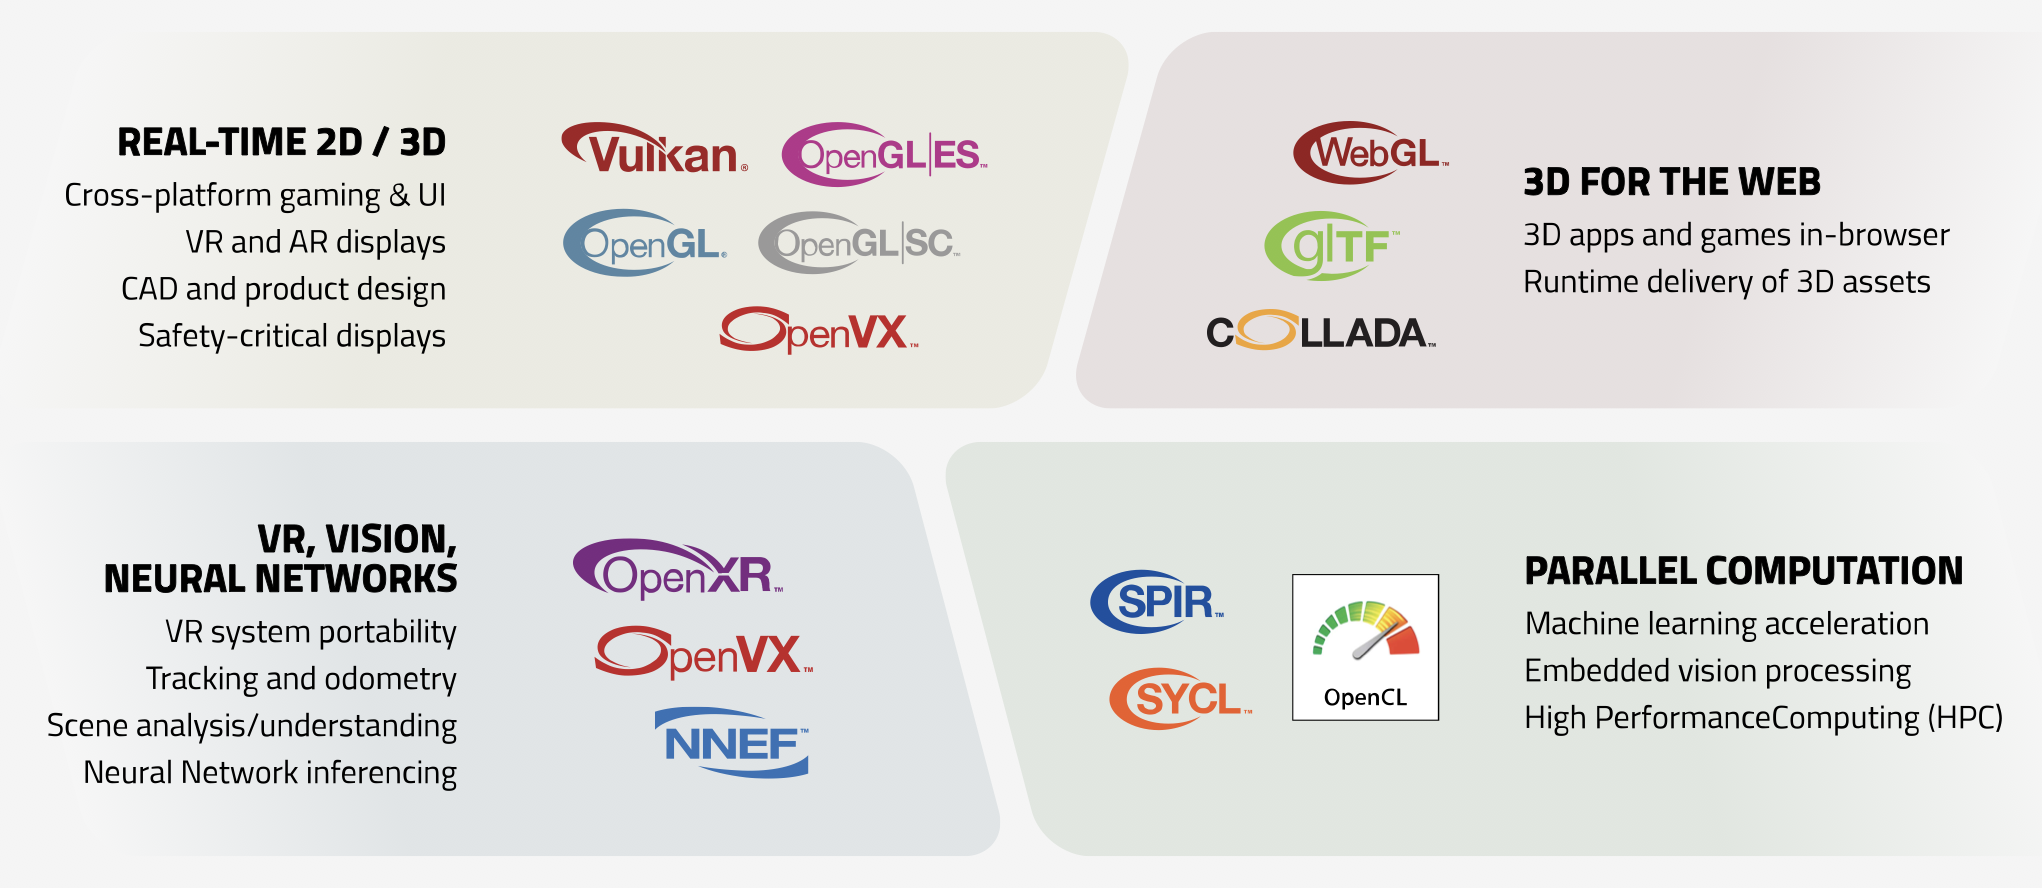
\includegraphics[width=0.8\linewidth]{Figures/khronos-visual-computing-ecosystem.png}
    \captionsource{Ecosystème des standards proposés par \textit{Khronos}}{khronos-ecosystem}
    \label{fig:khronos-visual-computing-ecosystem}
\end{figure}

\subsubsection{glTF}
\label{sec:glTF}

\textit{glTF} (\textit{\textbf{GL} \textbf{T}ransmission \textbf{F}ormat})\footnote{\url{https://www.khronos.org/gltf/}} est un standard ouvert défini par le \textit{Khronos Group}. Visant le même objectif que son prédécesseur \textit{COLLADA}, ce format a été optimisé au mieux pour réduire l'espace de stockage nécessaire pour les scènes ou modèles 3D représentés, tout en accélérant le chargement et traitement de ceux-ci. 
\textit{Khronos} le décrit comme le "JPEG de la 3D".
Ce format utilise \textit{JSON} pour décrire les données.

Bien que relativement récent (fin 2015), il a rapidement été adopté par les principaux acteurs du marché, et son acceptation continue de s'étendre. À titre d'exemple, \textit{Sketchfab} propose déjà plus de 100'000 modèles dans ce format\footnote{\url{https://blog.sketchfab.com/sketchfab-now-largest-online-repository-gltf-files/}} et a défini \textit{glTF} comme format d'exportation par défaut. Tous les modèles, quelque soit leur format d'origine, peuvent être convertis automatiquement dans ce format lors de leur téléchargement. 

\begin{figure}
    \centering
    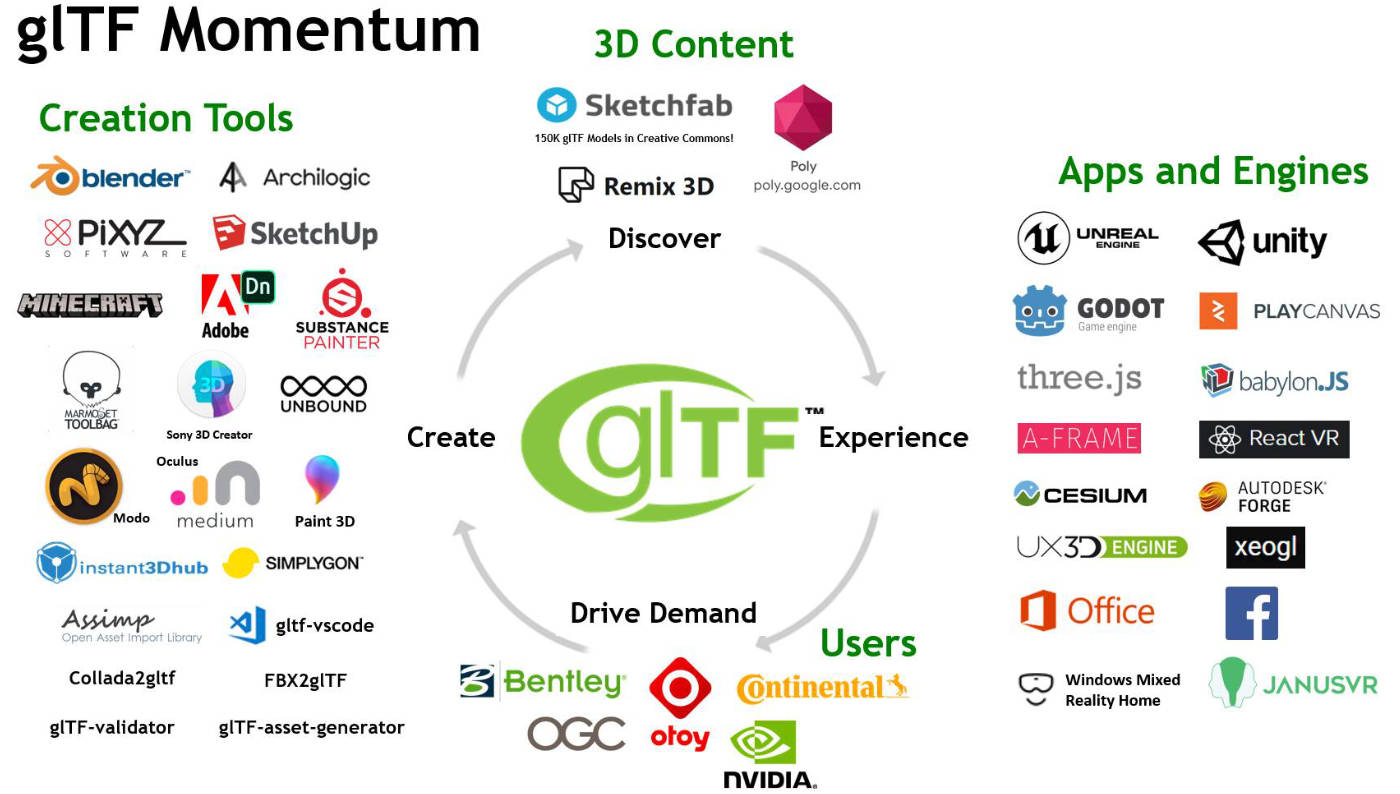
\includegraphics[width=0.8\linewidth]{Figures/gltf-momentum.jpg}
    \captionsource{Outils, applications, plateformes et sociétés employant \textit{glTF}}{gltf-momentum}
    \label{fig:gltf-momentum}
\end{figure}

\subsection{Gestion des fichiers dans le cadre du projet}

On imagine trois cas de figure :

La première possibilité, illustrée en \ref{fig:file-importation-process-native}, est de faire en sorte que l'outil sache lire les fichiers "tels quels", sans effectuer de réelles transformations.
L'avantage est que, pour autant que l'on ait implémenté le support du format de fichier fournit en entrée, celui-ci sera vraisemblablement rendu correctement. C'est un peu le principe des visionneuses d'images classiques, auxquelles on donne les instructions sur "comment lire tel ou tel format de fichier", et qui affichent correctement chaque pixel à l'écran.
Le problème de cette solution est qu'elle nécessite un travail conséquent. Pour qu'elle soit efficace, il faut implémenter bon nombre de formats, et qu'il faut être certain de bien avoir respecter les specifications.

\begin{figure}[ht]
    \centering
    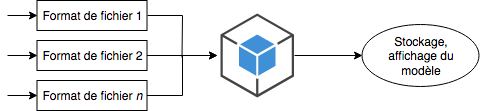
\includegraphics[width=\linewidth]{Figures/file-importation-process-native.png}
    \caption{Cas 1 : support natif des principaux formats}
    \label{fig:file-importation-process-native}
\end{figure}

Une variante est de définir un ou quelques formats principaux, complètement supportés par le logiciel. Si l'utilisateur souhaite importer un modèle stocké sous un format non pris en charge, il devra le convertir manuellement, par exemple à l'aide des fonctions d'exportation du logiciel utilisé pour sa conception.

\begin{figure}[ht]
    \centering
    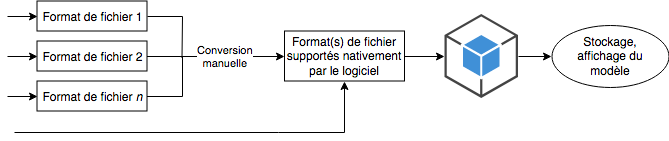
\includegraphics[width=\linewidth]{Figures/file-importation-process-manual-conversion.png}
    \caption{Cas 2 : conversion manuelle vers le(s) format(s) supportés}
    \label{fig:file-importation-process-manual-conversion}
\end{figure}

\begin{figure}[ht]
    \centering
    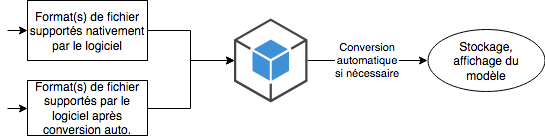
\includegraphics[width=\linewidth]{Figures/file-importation-process-auto-conversion.png}
    \caption{Cas 3 : conversion effectuée par le logiciel, si nécessaire}
    \label{fig:file-importation-process-auto-conversion}
\end{figure}


soit nativement (le logiciel sait lire différents formats), soit en se basant sur un format courant, vers lequel il est relativement aisé de convertir les autres types de fichiers au préalable.

\section{Système d'information géographique (SIG)}
Un \textit{SIG} est, comme son nom laisse supposer, un système d'information destiné à gérer des données spatiales ou géographiques. Il est difficile d'en donner une définition exacte, car les domaines concernés sont très vastes.

De manière générale, un \textit{SIG} sert à recueillir, stocker, analyser, éditer, partager et afficher lesdites données. Des outils sont mis à disposition des utilisateurs afin d'effectuer les tâches correspondantes, telles des requêtes sur les données.

Des exemples de SIG :

\begin{itemize}
    \item \textit{ArcGIS} de la société \textit{Esri}. C'est un ensemble complet de produits : du logiciel de bureau ou \textit{online}, en passant par des serveurs (managés ou hébergés chez \textit{Esri} ou encore sur un autre \textit{cloud}), ainsi que de nombreux outils de développement.
    \item \textit{QGIS} est un concurrent libre de \textit{ArcGIS}\footnote{Comparaison détaillée entre ArcGIS et QGIS (\textit{anglais, 2018}) : \url{https://gisgeography.com/qgis-arcgis-differences/}}
\end{itemize}

\section{Visionneuse de modèles 3D}

L'affichage et la manipulation de modèles 3D constitue la première brique d'un tel projet, la fondation sur laquelle viendront s'ajouter les modules complémentaires souhaités, tels que la création d'annotations, le stockage des modèles et des notes associées, etc.
Il existe de multiples visionneuses, qu'elles soient en ligne ou à installer. Le choix se réduit lorsque l'on recherche des projets open-source, ce qui était nécessaire de le cadre de ce projet : autant partir sur une base existante, et ne pas réinventer la roue.

\unsure{Suite à l'étude faite autour des formats de fichier, les recherches de visionneuses se sont limitées à celles supportant le format glTF.}

Parmi les projets open-source trouvé, nous nous sommes surtout intéressés à ceux actifs, c'est-à-dire ayant eu des activités récentes (mise à jour du code...). Parmi ces quelques-uns, voici les ceux qui auront retenus notre attention :

\begin{itemize}
    \item bwasty/gltf-viewer\footnote{\url{https://github.com/bwasty/gltf-viewer}} : développée en \textit{Rust}. Cette visionneuse est fonctionnelle, mais n'a pas été retenue d'une part car elle ne propose pas de version web, et d'autre part parce que je n'ai aucune expérience dans ce langage de programmation.
    \item pissang/clay-viewer\footnote{\url{https://github.com/pissang/clay-viewer}} : cette visionneuse permet de lire les fichiers \textit{FBX}, \textit{DAE} et \textit{OBJ}, et il est ensuite possible de les exporter au format \textit{glTF}. Les versions clients Windows et MacOS sont proposées. Très prometteur, ce projet n'a pas été retenu comme base pour deux raisons. La première, c'est qu'il n'est pas fait mention de version web - bien qu'en théorie, au vu des technologies utilisées (\textit{Javascript}, principalement), il serait possible de l'adapter. La seconde, c'est que le rendu est effectué à l'aide de ClayGL\footnote{\url{https://github.com/pissang/claygl}}, une librairie créée par le même développeur. Celle-ci est très prometteuse, maintenue activement à jour et commence à être utilisée dans quelques projets, mais n'est pas encore suffisamment répandue pour assurer que l'on trouvera suffisamment de documentation, exemples et aide en cas de besoin.
    \todo{propose un outil de conversion vers glTF, fait en python "ClayGL provide a python tool for converting FBX to glTF 2.0."}
\end{itemize}


Le choix s'est porté sur three-gltf-viewer.
Il s'agit d'un projet développé par un gars de chez Google, spécialisé dans...,  apparemment dans son temps libre.
Le projet a été démarré récemment (DATE) et toujours développé activement. Cela conforte dans l'idée que les technologies utilisées pour le concevoir soient modernes.

Les spécificités de ce projet sont détaillées sous "Langages et technologies".


\section{Langages et technologies}

Lorsque l'on se base sur un projet existant, l'une des contraintes et qu'il va falloir s'adapter aux technologies employées par celui-ci.

Un rapide tour d'horizon sur la page Github du projet, en activant l'affichage de la proportion d'utilisation de langages, nous apprend qu'il s'agit d'un projet web, composé essentiellement de JavaScript.

\begin{figure}[h]
    \centering
    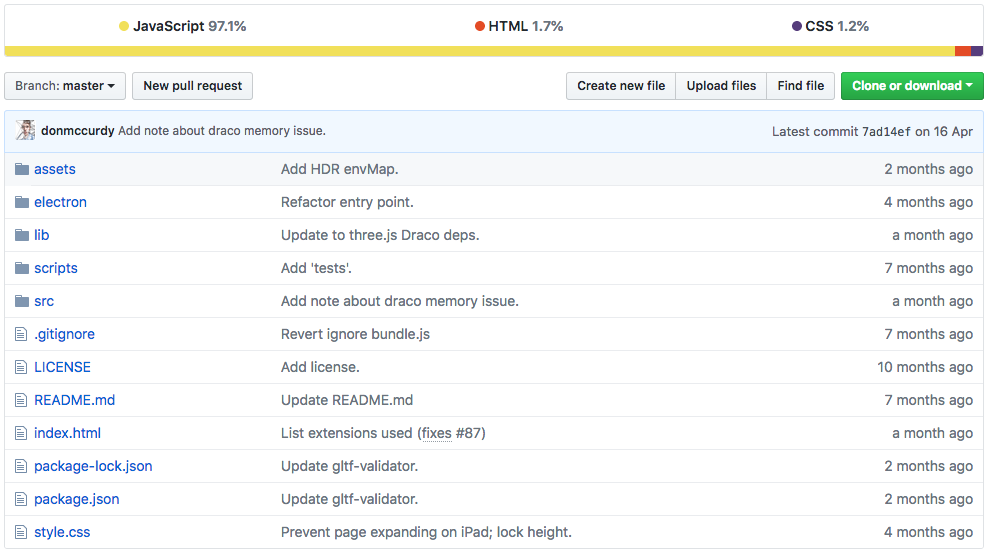
\includegraphics[width=\linewidth]{Figures/three-gltf-viewer-github-preview.png}
    \caption{Statistiques du projet three-gltf-viewer}
    \label{fig:three-gltf-viewer-github-preview}
\end{figure}

Les répertoires situées à la racine nous apprennent l'utilisation du framework Electron https://electronjs.org/.
\subsection{Electron}

\subsection{NodeJS}
Package.json -> Node...

Migration JS -> TS : \url{https://www.typescriptlang.org/docs/handbook/migrating-from-javascript.html}
malheureusement prendrai trop de temps dans le cadre de ce projet. On peut mixer du TS dans du JS mais c'est pas très simple...
Guide pour migrer une app React vers TS : \url{https://github.com/Microsoft/TypeScript-React-Conversion-Guide\#typescript-react-conversion-guide}

Javascript : cours J-L Falcone https://gitlab.unige.ch/courses/jsHepia

\subsection{WebGL}
\textit{WebGL} est une API, basée sur \textit{OpenGL}, servant à afficher des graphiques 2D et 3D dans tout navigateur web compatible\footnote{\url{https://caniuse.com/\#feat=webgl}}, à travers le \textit{canvas} d'\textit{HTML5}. 
Le rendu, au travers du langage \textit{GLSL}, est réalisé par le \textit{GPU}, fournissant ainsi d'excellentes performances. Ces dernières peuvent toutefois être limitées, par exemple sur des ordinateurs équipées d'anciennes cartes graphiques ainsi que les smartphones à la configuration plus modeste.

\textit{WebGL} est développé par le groupe \textit{Khronos}, le même à l'origine du format \textit{glTF} présenté en \ref{sec:glTF}.


\subsection{Three.js}
\textit{Three.js}\footnote{\url{https://threejs.org/}} est une librairie \textit{JavaScript} libre, permettant de créer et afficher des éléments 3D dans un navigateur. Très répandue




\section{Annotations}

Dans nos discussions de cas d'utilisation et de fonctionnalités(\ref{sec:use-cases}), pouvoir commenter et ajouter des informations à un modèle est un aspect qui a souvent été mentionné. C'est en effet une fonctionnalité importante pour toutes les catégories d'utilisateurs.

Dans le cadre d'une modélisation 3D, la particularité des annotations est d'être \textbf{associées à des coordonnées spécifiques} de celle-ci. Dans ce projet, c'est ce qui distingue les annotations de simples commentaires que l'on ajouterait en regard du modèle ou en dessous de celui-ci (comme des commentaires sur une photo ou une publication par exemple).

\subsection{Attributs d'une annotation}
Les données principales d'une annotation sont : son \textbf{contenu} et ses \text{information de localisation dans le modèle}.

Par contenu, on pense nécessairement à du texte, mais on peut aussi imaginer des images, des liens, une vue 360° prise à l'emplacement concerné, une vidéo, voire un autre modèle 3D (par exemple, de l'intérieur d'un bâtiment)...!

Dans \textit{Sketchfab}, les annotations ont un titre et une description. Cette dernière peut être rédigée en \textit{Markdown}; c'est de cette manière que l'on peut ajouter des liens et des images. Pour l'instant, la plateforme ne supporte pas les autres types de médias.

\begin{figure}
    \centering
    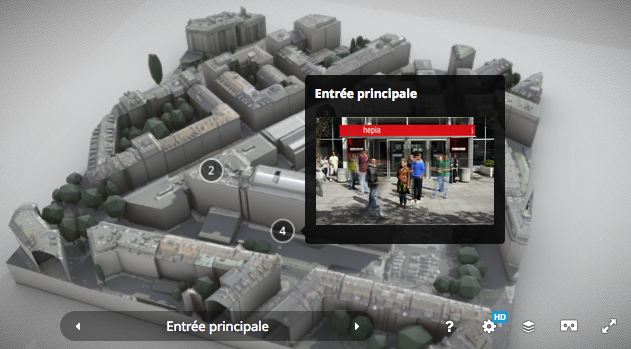
\includegraphics[width=\linewidth]{Figures/sketchfab-annotation-with-picture.png}
    \caption{Exemple d'annotation avec une image dans~\textit{Sketchfab}}
    \label{fig:sketchfab-annotation-with-picture}
\end{figure}

L'ajout d'une annotation dans Sketchfab se déroule ainsi : en mode édition, avec l'outil d'annotation actif, un double-clic sur le modèle affiche une fenêtre pour rédiger le contenu de l'annotation. Celle-ci est ensuite représentée par un cercle numéroté, qui reste à l'emplacement choisi, même lorsque l'on manipule le modèle (pivoter, déplacer...). 

\begin{figure}
    \centering
    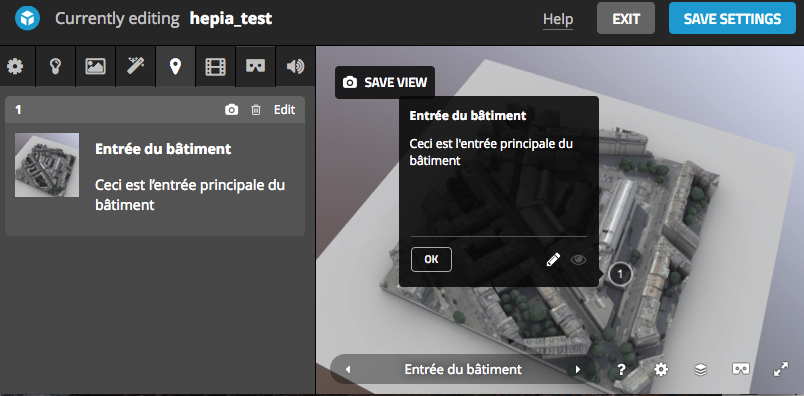
\includegraphics{Figures/sketchfab-adding-annotation.png}
    \caption{Exemple d'ajout d'une annotation en mode édition}
    \label{fig:sketchfab-adding-annotation}
\end{figure}

Au niveau technologique : les cercles sont des objets 3D ajoutés à la scène, généralement rendue en \textit{WebGL}. Le dialogue contenant l'annotation pourrait aussi être créé en \textit{WebGL}, mais \textit{HTML/CSS}  est bien mieux adapté pour tout ce qui a trait à la mise en page et aux typographies.

Parmi les fonctionnalités supplémentaires imaginées :


\todo{Images vues 360}

\todo{Concepts d'annotations : vue 360. naviguer dans une animation ? exemple : projet à plusieurs années d’intervalle, pouvoir bouger sur un curseur. \url{}}

\section{Stockage}
Stockage des modèles 3D :
plusieurs solutions sont envisageables. On pourrait utiliser une base de données spécifique aux SIG.
Une première implémentation serait faciliter par un simple stockage des fichiers à l'endroit d'exécution de l'application (sur son serveur p.ex.).


Stockage des annotations :
Format JSON

\subsection{GeoJSON}
\textit{GeoJSON} est un format ouvert,  basé sur JSON, développé pour représenter des caractéristiques géographiques.
Celles-ci incluent les points, les lignes et les polygones ainsi que des sous-ensembles de ces types. À ces éléments, on peut ajouter des attributs.



\section{Hébergement, déploiement}

\subsection{Déploiement en continu avec Heroku}

\textit{Heroku} est une Plateforme \textit{cloud} en tant que service (PaaS) qui offre l'infrastructure nécessaire au déploiement d'applications web. Ainsi, l'équipe de développement peut se concentrer sur le logiciel lui-même sans avoir à gérer la mise en place de serveurs, leur configuration etc.

Parmi les fonctionnalités proposées :
\begin{itemize}
    \item Possibilité de mettre à jour l'application automatiquement au moindre changement dans un \textit{repository} distant, par exemple si le projet est hébergé sur \textit{GitHub},
    \item Scalabilité des processus : en cas de montée en charge (augmentation du nombre de connexions, de traitements à effectuer...), le service offre la possibilité d'allouer des ressources supplémentaires
    \item Isolation : chaque processus est isolé des autres; ainsi si l'un pose problème, le reste du produit n'est pas impacté.
    \item Des logs complets et clairs pour dépanner efficacement son application,
    \item Une documentation vaste, de nombreuses ressources pour démarrer rapidement
\end{itemize}

\textit{Heroku} n'est évidemment pas la seule enterprise à proposer ce genre de services. Citons par exemple \textit{Amazon Web Services (AWS)}, \textit{Windows Azure} ou encore \textit{Google App Engine}.

\textit{Heroku} se démarque quelque peu de la concurrence grâce à la relative rapidité à laquelle on peut mettre en place une première application.


\subsubsection{Problèmes rencontrés}

Heroku considère que l'application se trouve à la racine du dossier.
Si l'application est située dans un sous-répertoire, l'une des possibilités est d'utiliser le module 'subtree' de git, qui permet de créer une sous-arborescence au sein d'un même projet. Ce dernier pourra alors être lié à une branche distincte, dans laquelle il se trouvera à la racine.
\begin{minted}{bash}
    git subtree push --prefix mysubtree origin subtree
\end{minted}

git subtree push --prefix mip-viewer origin heroku

Heroku est un environnement de production (pas de dev). Voir problème rencontré ici :

et commentaire :
Heroku is a production environment. The devDependencies are for packages that are required on your development environment only. Packages that you need to be included in your Heroku slug (including packages required during the slug build phase, such as webpack), need to be in your dependencies, not devDependencies. It is possible that you see people putting webpack in devDependencies for other platforms, but probably not for Heroku. 

et une possible solution étant de créer un script spécifique à Heroku : https://stackoverflow.com/a/42237745/1975002
Avantage : permet de ne pas faire grandir package.json, et d'isoler ce qui concerne Heroku.

Dans mon cas, comme seul le package 'webpack' était concerné, je l'ai "dédoublé" sous dependencies comme suggéré ici : https://stackoverflow.com/a/41973881/1975002

Heroku a pu ainsi faire une première build réussie de l'application. Celle-ci ne fonctionnait malheureusement pas encore correctement (voir \url{https://github.com/MichaelPolla/mip-viewer/issues/5\#issuecomment-390479224}) 
\chapter{Bilan et conclusion}
\label{Chapter4}

Ce projet a permis de définir une architecture modulaire possible pour une plateforme de modèles 3D dédiée ciblant le domaine de l'urbanisme.

Un tel outil 
%\include{Chapters/Chapter5} 

%----------------------------------------------------------------------------------------
%	THESIS CONTENT - APPENDICES
%----------------------------------------------------------------------------------------

\appendix % Cue to tell LaTeX that the following "chapters" are Appendices

% Include the appendices of the thesis as separate files from the Appendices folder
% Uncomment the lines as you write the Appendices

%\chapter{Structure du prototype réalisé}

\label{AppendixA}
% Bibliography documentation: 
% * https://fr.sharelatex.com/learn/Bibliography_management_with_bibtex
% * https://fr.wikibooks.org/wiki/LaTeX/Gestion_de_la_bibliographie



\begin{thebibliography}{9}

\footnotesize

\bibitem{plq-contest} Concours d’architecture sur le périmètre de la gare CEVA des Eaux-Vives: \\
\url{http://www.ville-geneve.ch/vie-quartier/eaux-vives-cite/actualites/detail-actualite/article/1397555164-concours-architecture-perimetre-gare-ceva-eaux-vives/}

\bibitem{wikipedia-3d-file-formats-list} Wikipédia - Liste des formats de fichiers 3D: \\
\url{https://en.wikipedia.org/wiki/List_of_file_formats\#3D_graphics}

\bibitem{overview-of-3d-data-content} \textit{"An Overview of 3D Data Content, File Formats and Viewers"}: \\
\url{https://www.archives.gov/files/applied-research/ncsa/8-an-overview-of-3d-data-content-file-formats-and-viewers.pdf}

\bibitem{xyz-format} Spécifications du format \textit{XYZ}: \\ \url{http://openbabel.org/wiki/XYZ_\%28format\%29}

\bibitem{mrc-format} Spécifications du format \textit{MRC}: \\ \url{http://www.ccpem.ac.uk/mrc_format/mrc2014.php}

\bibitem{fbx-api} API du format \textit{FBX}: \\
\url{https://www.autodesk.com/products/fbx/overview}

\bibitem{collada-format} Spécifications du format \textit{COLLADA}: \\
\url{https://www.khronos.org/collada}

\bibitem{collada-iso} Norme ISO/PAS 17506:2012 définissant le format \textit{COLLADA}: \\
\url{https://www.iso.org/standard/59902.html}

\bibitem{gltf-format} Spécifications du format \textit{glTF}: \\
\url{https://www.khronos.org/gltf/}

\bibitem{sketchfab-largest-gltf-repository} \textit{"Sketchfab is now the largest online repository of glTF files"}, 01.08.2017  \\
\url{https://blog.sketchfab.com/sketchfab-now-largest-online-repository-gltf-files/}

\bibitem{webgl-compatibility} Compatibilité de \textit{WebGL} avec les navigateurs: \\
\url{https://caniuse.com/\#feat=webgl}

\bibitem{geojson-rfc} RFC 7946 définissant le format \textit{geoJSON}: \\
\url{https://tools.ietf.org/html/rfc7946}

\bibitem{buildingsmart} Site de buildingSMART, à l'origine du standard \textit{openBIM}: \\
\url{https://www.buildingsmart.org/}

\vspace*{.06\textheight}
\textbf{Sources des images:}

\bibitem{3d-printed-model} \url{https://ge.ch/sitg/calendrier/espace-public/sig-3d-et-maquettes-987}

\bibitem{pav} \url{https://www.ge.ch/actualite/exposition-grande-maquette-du-projet-pav-3-05-2018}

\bibitem{khronos-ecosystem} \url{https://www.khronos.org/about/}

\bibitem{gltf-momentum}{\url{https://www.khronos.org/gltf/}}

\end{thebibliography}


%----------------------------------------------------------------------------------------
%	BIBLIOGRAPHY
%----------------------------------------------------------------------------------------

%\nocite{*}
%\printbibliography[heading=bibintoc]

%----------------------------------------------------------------------------------------

\listoftodos

\end{document}